%%%%%%%%%%%%%%%%%%%%%%%%%%%%%%%%%%%%%%%%%%%%%%%%%%%%%%%%%%%%%%%%%%%%%%%
% Universidade Federal de Santa Catarina             
% Biblioteca Universitária                     
%                                                           
% (c)2010 Roberto Simoni (roberto.emc@gmail.com)
%         Carlos R Rocha (cticarlo@gmail.com)
%%%%%%%%%%%%%%%%%%%%%%%%%%%%%%%%%%%%%%%%%%%%%%%%%%%%%%%%%%%%%%%%%%%%%%%
%\PassOptionsToPackage{abnt-etal-cite=1, abnt-etal-list=0}{abntcite}
\documentclass{ufscThesis}

\usepackage[page]{appendix}

%\usepackage{cite}
\usepackage{amsmath}
\usepackage{amssymb}
\usepackage{amsfonts}
\usepackage[utf8]{inputenc}
\usepackage{algorithmic}
\usepackage{algorithm}% http://ctan.org/pkg/algorithms
\usepackage{multicol}
\usepackage{amsthm}

\usepackage{mathtools}
\DeclarePairedDelimiter{\ceil}{\lceil}{\rceil}
\DeclarePairedDelimiter{\floor}{\lfloor}{\rfloor}
\newcommand{\minuseq}{\mathrel{{-}{=}}}
\newcommand{\F}{\mathbb{F}}
\newcommand{\primes}{\mathbb{P}}
\newcommand{\weight}[1]{\text{weight}({#1})}

\renewcommand{\algorithmicrequire}{\textbf{Input:}}
\renewcommand{\algorithmicensure}{\textbf{Output:}}
\renewcommand{\algorithmicforall}{\textbf{for each}}

\newcommand{\mathbox}[3][l]{\makebox[\widthof{$#2$}][#1]{$#3$}}

% From Elsevier class.
\newtheorem{thm}{Theorem}
\newtheorem{lem}[thm]{Lemma}
%\newdefinition{rmk}{Remark}
%\newproof{pf}{Proof}
%\newproof{pot}{Proof}

\newcommand{\specialcell}[2][c]{%
  \begin{tabular}[#1]{@{}l@{}}#2\end{tabular}}

% Without this the superscripts get too close to the upper line.
\renewcommand{\arraystretch}{1.2}
\setlength\tabcolsep{5mm}

\usepackage [english]{babel}
\usepackage [autostyle, english = american]{csquotes}
\MakeOuterQuote{"}


\newcommand{\ftwo}{{\mathbb F}_{2}}
\newcommand{\ftwom}{{\mathbb F}_{2^m}}
\newcommand\Tstrut{\rule{0pt}{2.1ex}}  

\newcommand{\rmv}[1]{}

\newcommand*\BitAnd{\mathrel{\&}}
\newcommand*\BitOr{\mathrel{|}}
\newcommand*\BitXOR{\mathrel{\oplus}}
\newcommand*\ShiftLeft{\ll}
\newcommand*\ShiftRight{\gg}
\newcommand*\BitNeg{\ensuremath{\mathord{\sim}}}


%%%%%%%%%%%%%%%%%%%%%%%%%%%%%%%%%%%%%%%%%%%%%%%%%%%%%%%%%%%%%%%%%%%%%%%
% Identificadores do trabalho
% Usados para preencher os elementos pré-textuais
%%%%%%%%%%%%%%%%%%%%%%%%%%%%%%%%%%%%%%%%%%%%%%%%%%%%%%%%%%%%%%%%%%%%%%%
% TODO: M mínusculo
\titulo{Fast modular reduction \protect\\ and squaring in $GF(2^\MakeLowercase{m})$} % Titulo do trabalho
%\subtitulo{Estilo \LaTeX~ padrăo}                % Subtitulo do trabalho (opcional)
\autor{Lucas Boppre Niehues}           % Nome do autor
\data{01}{Janeiro}{2017}                           % Data da publicaçăo do trabalho

\orientador{Prof. Ricardo Felipe Custódio}                    % Nome do orientador e (opcional) seu título
\coorientador{Prof. Daniel Panario}                % Nome do coorientador e seu título (opcional)
\coordenador{Prof. Chefe, Carina Dorneles}              % Nome do coordenador do curso e (opcional) seu título

\instituicao[o]{Universidade Federal de Santa Catarina}
\departamento[a]{Departamento de Informática e Estatistica}
\curso[o]{curso de Pós-Graduação em Ciência da Computação}
\grau{Mestre em Ciência da Computação}
\documento[a]{Dissertação}

%%% Sobre a Banca
\numerodemembrosnabanca{2} % Isso decide se haverá uma folha adicional
%\orientadornabanca{sim} % Se faz parte da banca definir como sim
%\coorientadornabanca{sim} % Se faz parte da banca definir como sim
\bancaMembroA{Primeiro membro da banca} %Nome do presidente da banca %TODO
\bancaMembroB{Segundo membro da banca}      % Nome do membro da Banca %TODO

\textoResumo {Resumo em portugues} %TODO

\palavrasChave {Corpos finitos, teoria de números, polinômios, squaring, criptografia.}

\textAbstract {We present an efficient bit-parallel algorithm for squaring in $GF(2^m)$ using polynomial basis. This algorithm achieves competitive efficiency while being aimed at any choice of low-weight irreducible polynomial. For a large class of irreducible polynomials it is more efficient than the previously best general squarer. In contrast, other efficient squarers often require a change of basis or are suitable for only a small number of irreducible polynomials. Additionally, we present a simple algorithm for modular reduction with equivalent cost to the state of the art for general irreducible polynomials. This fast reduction is used in our squaring method.}

\palavrasChave {Finite field, number theory, polynomial, squaring, cryptography.}

%%%%%%%%%%%%%%%%%%%%%%%%%%%%%%%%%%%%%%%%%%%%%%%%%%%%%%%%%%%%%%%%%%%%%%%
% Início do documento                                
%%%%%%%%%%%%%%%%%%%%%%%%%%%%%%%%%%%%%%%%%%%%%%%%%%%%%%%%%%%%%%%%%%%%%%%
\begin{document}
%--------------------------------------------------------
% Elementos pré-textuais
\capa  
\folhaderosto % Se nao quiser imprimir a ficha, é só năo usar o parâmetro
\folhaaprovacao
\paginaresumo
\paginaabstract
\listadefiguras
\listadetabelas 
\listadeabreviaturas
\listadesimbolos
\sumario

%Dissertação segundo papel de 2016/07/01
%%%%%%%%%%%%%%%%%%%%%%%%%%%%%
%1. Introdução:
%contexto
%objetivo - específico
%justificativa
%motivação
%conteúdo (na seção x...) 
%
%2. ref. teórico / introdução
%o que o leitor precisa saber para entender a tua proposta
%
%3. Proposta / O que fez!
%Artigo
%
%4. Disc. / Análise / comparação
%Do que foi feito
%
%5. Considerações finais
%Apanhado do que foi feito, linkado com objetivos específicos
%trabalhos futuros
%
%referências
%%%%%%%%%%%%%%%%%%%%%%%%%%%%%
\chapter{Introduction}
%% Contextualizar: do geral oara o específico, do que se trata o teu trabalho - 5 a 10 parágrafos contextualizando
% Qual é o problema, por que o problema é um problema
% Objetivos Geral e específicos
% Motivação
% Justificativa
% Metodologia de pesquisa adotada
% Opcional: listar as principais contribuicoes
% Opcional: Limitaçoes do teu trabalho, no sentido do que nao é o teu trabalho

% Motivação: por que trabalhar nesse tema. "trabalho de cooperação itnernacional labsec com a universidade de carleton, onde foram feitos vários trabalhos na área de processamento rápido de corpos finitos". aspeco social, pessoal, laboratório, pesquisa. "durante os anos as pesquisam sendo realizadas no grupo de pesquisas do labsec, chegou-se a conclusao que o desempenho e performance de algoritmos não era o desejado, com a vinda e internacionalização do grupo de pesquisa especial, e cooperação com a unviersidade de Carleton, descobriu-se que haviam alguams coisas a fazer..."
% Justificativa: científiac. É importante melhorar o desempenho pra trabalhar na aritmética em corpos finitos? Algoritmos são as peças chaves, diminuir úmero de operacóes leva a melhor performance...

% Näo incluir áreas de pesquisa que não deram resultado: shamir, ECC, etc. Se tiver alguma coisa na mesma área, incluir nos trabalhos futuros
Finite field arithmetic is the fundamental for many important cryptosystems, such as ECC (Elliptic Curve Cryptography). Such arithmetic is often implemented by performing operations on integers or polynomials, then performing modular reduction on the result. The usage of binary polynomials is specially common for hardware implementations, as the operations map well to logic gates.

The performance of such system is important because it maps directly to fabrication costs, circuit area, power consumption, and execution time. Since finite field arithmetic is the basis of various cryptosystems, any optimizations in this area will cause improvements in the general system. Such improvements are specially useful for constrained systems, such as sensor networks.

This work has two general objectives. First, to act as an introduction to finite field arithmetic, and how fields based on binary polynomials are used in practice, down to the logic gates. It is our hope that this introduction can help future researchers that wish to understand or improve this area.

Our second general objective is to propose improvements on finite field arithmetic, with the goal of having these low level improvements leading to improvements in the overall system. Specifically, reducing the delay and number of logic gates required for reduction and squaring in binary finite fields; generalizing these improvements to other finite fields implemented with polynomials; and finally, translating these low level improvements to software algorithms.

Our work was motivated by the international cooperation between our Universidade Federal de Santa Catarina, and the Canadian Carleton University. This cooperation produced many projects related to fast processing in finite fields, specifically for cryptographic systems. This choice of subject was the result of a general dissatisfaction of the speed of the high level systems. The approach of optimizing the low level components was seen as a natural consequence of the expertise brought by this cooperation.

In Chapter~\label{cap:background} we introduce the basic mathematics behind finite field, with a goal of both introducing the subject for interested researchers, and to give the necessary background for the subsequent chapters. We focus on reduction and exponentiation of binary polynomials, and propose new hardware algorithms in Chapter~\ref{chapters/reduction_squaring_2}. In Chapter~\ref{chapters/word_processing} we contextualize and provide tools on how to translate hardware algorithms in a way to also be efficient in software. Chapter~\ref{chapters/visual_debugger} showscases the visualization tools we developed to help this research. Chapter~\ref{chapters/final_considerations} contains our final considerations, giving a conclusion and raising interesting future works.


\section{Binary finite field arithmetic in ECC} \label{background:binary}

% Mais para um capítulo de introdução do que de background.
% Faltando estado da arte, faltando tabela.
% Avanços históricos, em relação da complexidade.

Arithmetic in the finite field $GF(2^m)$ of $2^m$ elements (also denoted $\F_{2^m}$) is fundamental for many important cryptosystems such as ECC (Elliptic Curve Cryptography). Such arithmetic is usually implemented by choosing an irreducible polynomial $f \in \F_2[x]$, $\deg(f) = m$, performing operations and reducing modulo this polynomial. It is common to have algorithms that implement arithmetic operations using a particular class of irreducible polynomials. This is because these algorithms are efficiently implemented considering such class of irreducibles.\\

Arithmetic operations in $GF(2^m)$ usually consist of addition (being equivalent to subtraction in characteristic 2), multiplication (of which squaring is a special case) and inverses. All these operations are used in ECC, making any optimizations reflect directly on the speed of elliptic curve arithmetic, raising the importance of choosing an irreducible polynomial and associated algorithms. As examples, the classes of pentanomials $x^m+x^{n+2}+x^{n+1}+x^{n}+1$, $x^{4s}+x^{3s}+x^{2s}+x^s+1$, $x^m+x^{m-r}+x^s+x^r+1$ and $x^m+x^{n+1}+x^n+x+1$ are used in fast multipliers~\cite{fan2015survey}, each with their own fast multiplication and reduction algorithms.\\

However, the algorithms designed for irreducible polynomials with specific exponents may contain internal structures with an unclear impact on security of applications that use these algorithms. No attacks have been demonstrated so far, but the security community has seen evidence of standards containing back doors~\cite{bernstein2016dual} and cryptography failing due to fixed parameters~\cite{adrian2015imperfect}. In light of these events there has been discussions for less magic parameters and more randomness in the structures used.\\

A related problem is that many classes of irreducible polynomials contain few elements with degrees interesting for instance for ECC, often having no irreducible polynomials at all for a desired degree. Furthermore, choosing a class to speed up a specific operation may lead to less efficient algorithms for other operations used in the same application. Choosing the parameters for a field is therefore an exercise in tradeoffs.

%\section{Objectives}
%
%General objectives:
%
%\begin{itemize}
%	\item Get introduced to finite field arithmetic.
%	\item Speed up cryptographic systems that depend on finite field arithmetic.
%\end{itemize}
%
%Specific objectives:
%
%\begin{itemize}
%	\item Create an efficient, general algorithm for binary polynomial reduction.
%	\item Create an efficient, general algorithm for binary polynomial squaring.
%	\item Translate speedups from hardware-oriented algorithms to software.
%\end{itemize}

% Introdução a finite fields
\chapter{Mathematical background}\label{cap:background}
%\section{Introduction}

For this work it is necessary to have a detailed understanding of finite fields, and how they implemented as primitives for higher level cryptographic structures. Here we focus on a specific type of field, polynomial fields. Furthermore, out of the possible representations we narrow our research to polynomial basis. \\

Finite fields have numerous applications in cryptography. We are mostly concerned with its use as low level primitive, and the performance of its arithmetic operations. One example of area that is benefited from this research is Elliptic Curve Cryptography, where the point computations are performed on fields such as the ones presented here. \\

This chapter is an introduction to the concepts that we will build upon. In Section~\ref{background:finite_fields} we explain the very basics of finite fields, trying to build an intuition of the structures involved. In Section~\ref{background:polynomial_representation} we focus on fields constructed from polynomials, and how to represent them. Section~\ref{background:arithmetic} explains the basics of arithmetic on binary polynomial basis, with some useful properties. Finally, Section~\ref{stateoftheart} shows the performance of state of the art algorithms for squaring and reduction. \\

\section{Finite fields} \label{background:finite_fields}

A Finite Field $\F_{p^m}$ (also known as Galois Field $GF(p^m)$) is an abstract mathematical structure composed of a set of elements and two operators: 

\begin{gather*}
\F_{p^m} = (\{A_0, A_1, A_2, ... A_{p^m-1}\}, +, \cdot),
\end{gather*}

where:

\begin{itemize}
\item $\F_{p^m}$: is a finite field of size $p^m$, where:
    \begin{itemize}
    \item $p$: the \emph{field characteristic}, $p \in \mathbb{P}$ (i.e. must be a prime number);
    \item $m$: the \emph{extension size} $m \in \mathbb{N^*}$ (i.e. $m \geq 1,~m$ integer);
    \end{itemize}
\item $\{A_0, A_1, A_2, ... A_{p^m-1}\}$: is a set of $p^m$ \emph{field elements}. In this work we use the letters $A$, $B$ and $C$ to refer to arbitrary members of this set, and $\F_{p^m}$ as an informal shorthand for this set (e.g. $A \in \F_{p^m}$).
\item $+, \cdot$~: are addition and multiplication operators, where:
    \begin{itemize}
    \item they are binary operators that operate on field elements, $+, \cdot : (\F_{p^m} \times \F_{p^m}) \mapsto \F_{p^m}$;
    \item there are two elements labeled $0$ and $1$ that behave as the additive and multiplicative identities, $0 \neq 1$, such that $\forall A (A + 0 = A~\wedge~A \cdot 1 = A)$;
    \item both operations commute (i.e. $A + B = B + A$ and $A \cdot B = B \cdot A$) and associate (i.e. $(A + B) + C = A + (B + C)$ and $(A \cdot B) \cdot C = A \cdot (B \cdot C)$);
    \item every element has an additive and a multiplicative inverse, also in the field (i.e. there are elements $-A$ and $A^{-1}$ such that $A + (-A) = 0$ and $A \cdot A^{-1} = 1$);
    \item except the multiplicative identity $0$, which has no multiplicative inverse (i.e. $0^{-1}$ is undefined);
    \end{itemize}
\end{itemize}

All fields of the same size are isomorphic, and therefore a field can be uniquely identified by its size. There are many ways to construct a field, with modular arithmetic being a common one. Finite fields are commonly constructed using integer arithmetic when $m=1$ (e.g. $\F_{13}$) or polynomial modular arithmetic otherwise (e.g. $\F_{2}[x]/(x^7+x^4+1)$.\\

Take for example the field $\F_{13}$ ($p=13,~m=1$). Fields with $m=1$ must have a prime number of elements, and are commonly called \emph{prime fields}. In the case $\F_{13}$, it can be constructed as $(\{0, 1, 2, ... 11, 12\}, +, \cdot)$. In this field, addition and multiplication are the usual operations, but always modulo the field size, $13$. Therefore:

\begin{align*}
5 + 10 &\equiv 2 \mod 13 \\
5 \cdot 4 &\equiv 7 \mod 13 \\
\end{align*}

Subtraction and division are performed using the additive and multiplicative inverses. Subtration is based on values of the format $-A$, where $A + (-A) \equiv 0 \pmod p$ in prime fields. The multiplicative inverse has an analogous property, where $A^{-1}$ is defined by $A \cdot A^{-1} \equiv 1 \mod p$. For example, $5^{-1} = 8 \mod 13$ because $5 \cdot 8 \equiv 1 \mod 13$. With these two definitions it's possible to define subtraction as $A - B = A + (-B)$, and division as $A / B = A \cdot B^{-1}$.

\section{Polynomial representation} \label{background:polynomial_representation}

For finite fields $\F_{p^m}$ with $m > 1$, one possible structure is to use polynomials of degree $<m$, where coefficients in $\F_{p}$. For instance, the element $A$ can be represented as $\sum_{i=0}^{m-1} a_i x^i,~a_i \in \F_{p}$. Then we choose an \emph{irreducible polynomial} $f$, of degree $m$ and coefficients in $\F_{p}$, and results are taken modulo $f$.\\

The concept of irreducible polynomials is analogous to the primality of integers. A polynomial is \emph{irreducible} if it has degree larger than $2$, and cannot be factored into the product of two other polynomials of degree larger than $2$. It can be thought as a polynomial with no non-trivial divisors.\\

The standard notation for fields using modular arithmetic with irreducible polynomials is $\F_p[x]/f$, where $\F_p[x]$ represents polynomials with coefficients in $\F_p$ and variable $x$, while $/f$ means that operations are performed modulo the irreducible polynomial $f$. As an example of a polynomial representation, the field $\F_{2^7}$ ($p=2,~m=7$) can be constructed as:

\begin{gather*}
\F_{2}[x]/(x^7+x^4+1) = (\{0, 1, x, x+1, x^2, x^2+1, x^2+x, \\
\hspace{8mm} \ldots~, x^6+x^5+x^4+x^3+x^2+x+1\}, +, \cdot)
\end{gather*}

In this case, addition is performed as usual for polynomials, but with the coefficients in $\F_2$:

$$(x^2+x+1) + (x+1) = (x^2+2x+2) \equiv (x^2)$$.

Note that no modulo operation, or \emph{reduction}, is required for additions. This is because the degree of $A+B$ is at most the of $A$ or the degree of $B$. Multiplications, on the other hand, may require reduction modulo $f$ (e.g. $f=x^7+x^4+1$ in this example):

$$(x^4+1) \cdot (x^3+x^2+x+1) \equiv (x^6+x^5+x^3+x^2+x) \mod (x^7+x^4+1)$$.

\section{Arithmetic in finite fields} \label{background:arithmetic}

The choice irreducible polynomial doesn't affect the algebraic structure, since it is isomorphic to any other representations of $\F_{p^m}$. However, certain polynomials have properties that may lead to simplifications in the field operations, making them of high interest for fast implementation in hardware or software.\\

In this work, we focus on polynomial representations of finite fields, with $p=2$ unless noted (e.g. $\F_{2^m}$). They are specially interesting for computations because the coefficients can be thought of as bits, and each element as an array of their coefficients. For example, for an arbitrary element $A$ we can represent it as a sequence of bits with the following notation:

\begin{align*}
A(x) &= x^6+x^3+x \\
& = 1x^6+0x^5+0x^4+1x^3+0x^2+1x+0\\
& \rightarrow [1, 0, 0, 1, 0, 1, 0] \\
\\
A &= [a_{m-1}, a_{m-2}, ..., a_2, a_1, a_0] \\
\end{align*}.

This representation is named \emph{polynomial basis}. In this view, a field addition is just a bitwise XOR operation. For example, the addition of two polynomials $(x^5+x^2)+(x^2+1)$:

\begin{gather*}
(x^5+x^2)+(x^2+1) \rightarrow [0, 1, 0, 0, 1, 0, 0] \oplus [0, 0, 0, 0, 1, 0, 1] \\
= [0, 1, 0, 0, 0, 0, 0],
\end{gather*}

and a multiplication can be performed by a regular polynomial multiplication followed, if needed, by a reduction operation. This $\texttt{reduce}_f$ function takes a "double wide" polynomial (because the resulting degree can be up to $2m-2$), which is not reduced representation of a field element, and returns the reduced representation (the product):

\begin{gather*}
C = A \cdot B\\
D \equiv C \mod f\\
\\
(x^6+1) \cdot (x^3+x^2+x+1) = x^9 + x^8 + x^7 + x^6 + x^3 + x^2 + x + 1 \\
\texttt{reduce}_f([0, 0, 0, 1, 1, 1, 1, 0, 0, 1, 1, 1, 1]) \rightarrow [0, 1, 0, 1, 1, 1, 1, 0]\\
\equiv x^6 + x^4 + x^3 + x^2 + x \mod x^7+x^4+1
\end{gather*}

This function, $\texttt{reduce}(C, x^m+...+1) = D$ is the main focus of this work, as it is generalized and used for efficient exponentiations.


\section{State of the art} \label{stateoftheart}

Algorithms for reduction and squaring in binary fields usually require only bitwise XOR operations. Their efficiency is then measured by a function of $m$, for irreducible polynomials of a certain class. Additionally, circuit algorithms are concerned with the critical path delay, measured as the number of XOR operations found in the longest path in the circuit. \\

For example, Table~\ref{table:comparison_squarer_background} compares the efficiency of two algorithms from the literature. The algorithms are optimized for small subsets of all irreducible pentanomials, thus the total number of suitable polynomials that exist. \\

\begin{table}
\centering
\caption{$GF(2^m)$ squarers for $x^m + x^a + x^b + x^c + 1$ in polynomial basis, $m > a > b > c > 0$, $m < 800$, $m$ prime, $\beta = \max{\{a, b, c, 0\}}$ such that $\beta \not \equiv m \pmod{2}$. Compare to results from Hariri \cite{hariri2009bit} and Park \cite{park2012explicit}}
{\begin{tabular}{l r l}
\label{table:comparison_squarer_background}
Proposal / Polynomials & \# irreducible & XOR count / Delay  \\ \hline
\specialcell{Hariri \\ $a=b+1=c+2$} & \specialcell{$602$} & \specialcell{$(m-3)/2 + m + 4$ \\ $2T_X$} \\ \hline
\specialcell{Park \\ $a \leq \ceil{m/2}$} & \specialcell{$2,011,941$}& \specialcell{$\leq (3m+7a-b-3c+25)/2$ \\ $3T_X$} \\ \hline
\end{tabular}}{}
\end{table}

Another class of interesting reduction algorithms are the ones that operate on NIST polynomials. NIST is the American National Institute of Standards and Technology, and is known for promoting cryptographic standards such as preferred finite fields for elliptic curves. \\

Because these fields are standardized, they attract special attention from researchers looking to optimize arithmetic operations. The state of the art for squaring modulo a NIST pentanomial, for example, is from Park \cite{park2012explicit}. The performance of the algorithm is available at Table~\ref{table:comparison_nist_background}, and a comparison to naive reduction.

\begin{table}
\centering
\caption{Squarer cost for NIST suggested ECC irreducible pentanomials, in number of XOR operations and circuit delay, where "naive reduction" is Algorithm~\ref{alg:reduce}.}
{\begin{tabular}{l r r} \label{table:comparison_nist_background}
Polynomial & Naive reduction & Park \cite{park2012explicit} \\ \hline
$x^{163} + x^7 + x^6 + x^3 + 1$ & $648\oplus/~5T_X$ & $246\oplus/~3T_X$ \\ \hline
$x^{283} + x^{12} + x^7 + x^5 + 1$ & $1,118\oplus/~5T_X$ & $\leq468\oplus/~\leq3T_X$  \\ \hline\
$x^{571} + x^{10} + x^5 + x^2 + 1$ & $2,280\oplus/~4T_X$ & $\leq898\oplus/~\leq3T_X$
\end{tabular}}{}
\end{table}

And for word-level reduction algorithms, Hankerson~\cite[p. 76]{hankerson2006guide} published the following results:

\begin{itemize}
\item $x^{163} + x^7 + x^6 + x^3 + 1$: 41 XORs, 36 SHIFTs, 1 AND = 78 operations
\item $x^{233} + x^{74} + 1$: 35 XORs, 35 SHIFTs, 1 AND = 71 operations
\item $x^{283} + x^{12} + x^7 + x^5 + 1$: 76 XORs, 76 SHIFTs, 1 AND = 153 operations
\item $x^{409} + x^{87} + 1$: 54 XORs, 54 SHIFTs, 1 AND = 109 operations
\item $x^{571} + x^{10} + x^5 + x^2 + 1$: 148 XORs, 148 SHIFTs, 1 AND = 297 operations
\end{itemize}

% Artigo rejeitado para IEEE (https://www.sharelatex.com/project/56e84e3540deb4e636bf5aab)
\chapter{Reduction and Squaring in $GF(2^\MakeLowercase{m})$}
%\section{Introduction}

Arithmetic in the finite field $GF(2^m)$ of $2^m$ elements (also denoted $\F_{2^m}$) is fundamental for many important cryptosystems such as ECC (Elliptic Curve Cryptography). Such arithmetic is usually implemented by choosing an irreducible polynomial $f \in \F_2[x]$, $\deg(f) = m$, performing operations and reducing modulo this polynomial. It is common to have algorithms that implement arithmetic operations using a particular class of irreducible polynomials. This is because these algorithms are efficiently implemented considering such class of irreducibles.\\

Arithmetic operations in $GF(2^m)$ usually consist of addition (being equivalent to subtraction in characteristic 2), multiplication (of which squaring is a special case), and multiplicative inverses, used in divisions. All these operations are used in ECC, making any optimizations reflect directly on the speed of elliptic curve arithmetic, raising the importance of choosing an irreducible polynomial and associated algorithms. As examples, the classes of pentanomials $x^m+x^{n+2}+x^{n+1}+x^{n}+1$, $x^{4s}+x^{3s}+x^{2s}+x^s+1$, $x^m+x^{m-r}+x^s+x^r+1$ and $x^m+x^{n+1}+x^n+x+1$ are used in fast multipliers, each with their own fast multiplication and reduction algorithms. See \cite{fan2015survey} for a comprehensive survey on this.\\

However, the algorithms designed for irreducible polynomials with specific exponents may contain internal structures with an unclear impact on security of applications that use these algorithms. No attacks have been demonstrated so far, but the security community has seen evidence of standards containing back doors~\cite{bernstein2016dual} and cryptography failing due to fixed parameters~\cite{adrian2015imperfect}. In light of these events there has been discussions for less magic parameters and more randomness in the structures used.\\

A related problem is that many classes of irreducible polynomials contain few elements with degrees interesting for instance for ECC, often having no irreducible polynomials at all for a desired degree. Furthermore, choosing a class to speed up a specific operation may lead to less efficient algorithms for other operations used in the same application. Choosing the parameters for a field is therefore an exercise in tradeoffs. \\

In this chapter we introduce a general algorithm for $GF(2^m)$ modular reduction and an efficient squarer suitable for \emph{any} low-weight irreducible polynomial $f$. These algorithms operate on elements represented in polynomial basis, where the coefficients are stored simply as an array of bits, and operations are performed bitwise in a logic circuit. Such algorithms are usually measured by the number of bit-level XOR operations performed and their circuit delay (we note that only XOR operations are required in these algorithms). Previous works on this operation have been limited to certain classes of irreducible polynomials to achieve competitive efficiency, fixing the weight (number of non-zero elements) and the relationship among exponents. 
Although our algorithms hold for any low-weight polynomial, to achieve better circuit delay and be more comparable to other proposals, we focus on the pentanomial case $x^m+x^a+x^b+x^c+1$, $m > a > b > c > 0$, where $a \leq \ceil{m/2}$.\\

Our squarer has different costs depending on the irreducible polynomial used. Applications requiring utmost efficiency should choose an irreducible polynomial to minimize the global cost of operations. We observe there are polynomials that minimize the number of XOR operations and delay with our squarer; we show that low-weight polynomials with this characteristic are abundant (see Table~\ref{table:comparison_squarer} in Section~\ref{comparison}). Additionally, our squarer can be used for higher weight polynomials, with some performance penalty.\\

The structure of the next sections is as follows. In Section \ref{modrec}, we present a general algorithm to perform modular reduction. This algorithm is generic and can be used with any irreducible polynomial. In Section \ref{squaring}, we modify the algorithm previously proposed to make it a squarer. This strategy allowed us to propose a squarer algorithm of low complexity. In Section \ref{comparison}, we compare our squarer with previous methods for this operation. Section~\ref{pth} shows how the reduction and squaring algorithm can be generalized for $p$-th power computation in characteristic $p$. \\

\section{Modular reduction} \label{modrec}

Let $GF(2^m)$ be a finite field generated by an irreducible polynomial $f(x) = x^m + r(x)$, where $\deg(r) < m$. Some polynomial basis operations performed on this field may require a reduction modulo $f$. This is a classical operation; see for example \cite[Chapter~2.3.5]{hankerson2006guide}.\\

Let $C(x) = \sum_{i=0}^{d} c_i x^i$, $d \geq m$, be the result of an operation before the reduction mod $f$ is executed. A simple method for reduction consists of iteratively computing $C(x) \leftarrow C(x) + c_{i} x^{i-m} f(x)$ for $i = d, d-1, \ldots, m$, where each step $i$ reduces the coefficient $c_{i}$.\\

To reduce the number of operations we replace $c_{i} x^{i-m} f(x)$ with $c_{i} x^{i-m} r(x)$ in the equation above, and then compute the final result mod $x^m$, which is a simple truncation. This avoids one XOR per iteration because $r$ has one less coefficient than $f$. We consider the truncation to have negligible cost. Algorithm~\ref{alg:reduce} is a pseudocode representation of these operations. The input consists of $d+1$ signals (the input coefficients), which are modified using XOR operations and returned as $m$ signals. We describe the details of this algorithm since it is a step in the construction of the main contribution in this chapter: the squarer method given in the next section. \\

\begin{algorithm}
\caption{General modular reduction for $GF(2^m)$}
\label{alg:reduce}
\begin{algorithmic}[1]
\REQUIRE $C = [c_0, c_1, c_2, ..., c_d]$, $d \geq m$, $f(x) = x^m + r(x)$
\ENSURE $C \pmod f$
\FOR{$i = d, d-1, \ldots, m$}
\FORALL{exponent $e$ \textbf{of} $r$}
\STATE $C[i-m+e] \leftarrow C[i-m+e] \oplus C[i]$ \label{alg:reduce:op}
\ENDFOR
\ENDFOR
\RETURN $C[0],~C[1],~C[2],~\ldots,~C[m-1]$
\end{algorithmic}
\end{algorithm}

Algorithm~\ref{alg:reduce} uses $(d-m+1)w_r$ XOR operations, where $w_h$ is the weight of the polynomial $h$, that is, the number of non-zero terms. If $C$ is a product of two polynomials of degree at most $m-1$, then the degree of $C$ is at most $d \leq 2m-2$. It is common, in practical implementations, to fix $d=2m-2$. In this case, the number of XOR operations to perform a modular reduction for trinomials and pentanomials are $2m-2$ and $4m-4$, respectively. The trinomial algorithm can be trivially modified to the equally spaced case, $x^m+x^{m/2}+1$, for $m$ even, where many operations cancel themselves out and result in $1.5 m - 1$ XOR operations~\cite{wu2002bit}.\\

The delay of Algorithm~\ref{alg:reduce} depends on the exact polynomial used, ranging from $2 T_X$ to $(m-1) T_X$, where $T_X$ is the delay of a single XOR gate. Unfortunately, the delay has no clear pattern in our algorithm. For the pentanomial case with $a \leq \ceil{m/2}$, we have empirically observed the following relation in irreducible pentanomials of degree up to 800, $m$ prime (see Table~\ref{table:reduce:delays} for statistical breakdown):

\[
    \text{delay}(a, b, c)= 
\begin{cases}
    6 T_X, & \text{if } c > \ceil{a/2}; \\
    5 T_X, & \text{if } \ceil{a/2} \geq c > \min(\ceil{b/2}, a-b+1); \\
    4 T_X, & \text{otherwise.}
\end{cases}
\]

\begin{table}
\centering
\caption{Circuit delay of Algorithm~\ref{alg:reduce} for irreducible pentanomials $x^m + x^a + x^b + x^c + 1$, $m < 800$, $m$ prime, $a \leq \ceil{m/2}$.}
{\begin{tabular}{l l l} \label{table:reduce:delays}
Delay & \# pentanomials & Percentage \\ \hline
$4 T_X$ & $694,789$ & $34.53\%$ \\ \hline
$5 T_X$ & $826,066$ & $41.06\%$ \\ \hline 
$6 T_X$ & $491,096$ & $24.41\%$ \\ \hline
All & $2,011,941$ & $100\%$
\end{tabular}}{}
\end{table}

Higher values of delay are observed when $a > \ceil{m/2}$. This trend can also be seen in other algorithms~\cite{fan2015survey}, and it is likely a consequence of the number of reduction steps~\cite{wu2002bit}. This means that for low delay reduction of products it is preferable to have irreducible polynomials where the second highest exponent is less than half of the degree $m$.\\

For the rest of this chapter we focus on pentanomials with $d=2m-2$ and $a \leq \ceil{m/2}$.

% \textbf{Algoritmo de redução de trinômios equally spaced?}

% \textbf{Texto sobre delays está comentado.}
%The bit operations are parallelizable, with a critical path of length $$\left \lfloor \frac{d-m}{m-\deg(r)} \right \rfloor + 1 .$$ The circuit delay is then the critical path length times the delay of a single XOR gate, $T_X$.

%When $d=m$ or $d=m+1$ the delay is always $1 T_X$, regardless of $\deg(r)$. For values of $d$ between $m+2 \leq d \leq 2m-2$ a delay of $1 T_X$ is only possible when $d + \deg(r) < 2m$. A delay of $1 T_X$ is not possible for $d > 2m-2$.

%We note that the delay is $2T_X$ if $$2m-d~\leq~\deg(r)~<~\frac{3m-d}{2},$$ and therefore only possible when $m+2 \leq d < 3m-2$.

% This particular case has been treated in the literature; a delay of $1 T_X$ is only achievable for irreducible trinomials $x^m+x+1$, and a delay of $2 T_X$ happens for any irreducible polynomial where $\deg(r) \leq \ceil{m/2}$.

%In practice $d$ is taken to be $2m-2$, the size of a product between two polynomials of degree $m-1$.

% \textbf{Mostrar dedução das desigualdades em um ou dois passos. "We can have other $T_X$". Mencionar que $2 T_X$ só é possível . "Portanto, existem muitos valores de $d$, dado $m$, tal que o polinômio $r(x)$ existe e o delay é $\leq 2 T_X$". "The particular case $d=2m-2$ has been treated in the literature, and in this case $r(x)$ must be..."}

\section{Squaring} \label{squaring}

Given an element $A(x) = \sum_{i=0}^{m-1} a_i x^i$ in $GF(2^m)$, computing its square is usually cheaper than naively multiplying $A$ by itself~\cite{fan2015survey}. For instance, using normal basis, a squarer is just a shift, but this basis is avoided in many situations due to the higher cost of multiplications using this type of  basis~\cite{fan2015survey}.\\

Algorithm~\ref{alg:reduce} can be modified to perform fast squaring operations in polynomial basis by setting $d=2m-2$ and using the property that $A^2 = \sum_{i=0}^{m-1} a_i x^{2i}$. Therefore, $A^2$ can be computed by interspacing zeroes between the coefficients of $A$, followed by a modular reduction, if necessary~\cite{wu2002bit}. The new algorithm is shown in Algorithm~\ref{alg:square}. The placing of zeroes is considered to have negligible cost on a logical circuit, hence the complexity of our squarer is restricted by the complexity of performing the modular reduction of $A^2$.\\

In Algorithm~\ref{alg:reduce} the operation $C[i-m+e] \leftarrow C[i-m+e] \oplus C[i]$ on Step~\ref{alg:reduce:op} performs one XOR and modifies one coefficient. When applied to $A^2$, each operation falls into one of three cases, depending on the parity of the indexes, and if the coefficients have been modified by a previous operation. In the following we analyze these three cases. \\

\begin{description}
\item[Case 1:] $i$ is odd and $C[i]$ has not yet been modified, therefore $C[i]=0$, and the operation has no effect.
    
\begin{lem} \label{lemma:case1}
Let $\beta$ be the highest exponent of $r$ such that $\beta \not\equiv m \pmod {2}$. Case 1 above allows for $(m-1-\beta) / 2$ coefficients to be skipped.
\end{lem}

\begin{proof}
The bits of $C$ are modified at the index $i-m+e$. The highest possible odd index for $i-m+e$ is $m-2+\beta$, when $i=2m-2$ (first iteration) and $e = \beta$. Therefore all bits at odd indexes greater than or equal to $m+\beta$ are known to be zero and are never modified (Case 1). This skips $\left((2m-2) - (m+\beta) + 1\right)/2 = (m-1-\beta)/2$ iterations. Additionally, these bits are never used and can be omitted from the circuit.
\end{proof}

\item[Case 2:] $i-m+e$ is odd and $C[i-m+e]$ has not yet been modified, therefore $C[i-m+e]=0$, no XOR is required, and only the copy $C[i-m+e] \leftarrow C[i]$ is necessary.
    \begin{lem} \label{lemma:case2}
Case 2 above allows for $(m-1+\beta)/2$ XOR operations to be replaced with a simpler copy operation.
\end{lem}

\begin{proof}
The first time an odd coefficient is modified, the XOR and assignment operation can be replaced with a simple assignment since the previous value is known to be zero (Case 2). There are $m-1$ odd coefficients, of which $(m-1-\beta)/2$ are skipped per Lemma~\ref{lemma:case1}. The total number of XOR operations avoided in this case is then $(m-1+\beta)/2$.
\end{proof}

\item[Case 3:] Otherwise, the operation continues normally and XORs are performed.
\end{description}

\vspace{2mm}

Using the savings provided by Lemma~\ref{lemma:case1} and Lemma~\ref{lemma:case2} we can give the total cost of squaring using Algorithm~\ref{alg:reduce}.

\begin{thm} \label{theorem}
Polynomial basis squaring in $GF(2^m)$ can be computed in $(w_r-1) (m-1+\beta)/2$ XOR operations.
\end{thm}

\begin{proof}
    Algorithm~\ref{alg:reduce} can be used to perform a modular reduction of $A^2$ in $(m-1)w_r$ XOR operations. Lemma~\ref{lemma:case1} allows for $(m-1-\beta)/2$ coefficients to be skipped, saving $w_r$ XORs each. Furthermore Lemma~\ref{lemma:case2} avoids another $(m-1+\beta)/2$ XOR operations. Hence we can reduce the number of XOR operations by a total of $w_r (m-1-\beta)/2 + (m-1+\beta)/2$. The total number of operations is then $$(m-1)w_r - w_r (m-1-\beta)/2 - (m-1+\beta)/2 = (w_r-1) (m-1+\beta)/2.$$ The interspacing of zeroes, simple assignments and final truncation are considered to have negligible cost.
\end{proof}

Algorithm~\ref{alg:square} performs the zero interspacing and uses the above cases to reduce the number of operations during the reduction. The internal variable $S$ keeps track of which coefficients have been assigned and therefore which case is applicable. The algorithm ends with a truncation mod $x^m$ as in Algorithm~\ref{alg:reduce}. We note the case analysis depends only on the irreducible polynomial $f$ and can be precomputed, resulting in a list of simple assignments and XOR operations with fixed indexes. \\

By Theorem~\ref{theorem}, the total number of XOR operations performed in Algorithm~\ref{alg:square} is $(w_r-1) (m-1+\beta)/2$. This is equivalent to the state of the art for trinomials~\cite{wu2002bit}, but we observe our algorithm holds for irreducible polynomials of any weight. When using irreducible pentanomials the cost ranges from $1.5(m-1)$ when $\beta=0$ (all exponents odd except the independent term) to $3(m-1)$ when $\beta=m-1$. \\

For irreducible septanomials the cost of squaring is $2.5(m-1+\beta)$ XORs. This is interesting as a low $\beta$ septanomial can be more efficient than a high $\beta$ pentanomial. Unfortunately, there has been little research for septanomials and higher weights, therefore we focus on pentanomials for this chapter. \\

Having $\beta=0$ implies $m$, $a$, $b$ and $c$ are odd, and such irreducible pentanomials are plentiful. If the exponents of the pentanomial were randomly distributed, it is expected that about $12.5\%$ of the odd degree pentanomials would have $\beta=0$. We enumerate all irreducible binary pentanomials with $m < 800$, $m$ a prime number (a common assumption in ECC \cite{doche2005redundant}), $a \leq \ceil{m/2}$ (for low delay), and observe $2,011,941$ meet this restriction. \\

\begin{algorithm}
\caption{General squaring for $GF(2^m)$}
\label{alg:square}
\begin{algorithmic}[1]
\REQUIRE $A = [a_0, a_1, a_2, ..., a_{m-1}]$, $f(x) = x^m + r(x)$
\ENSURE $A^2 \pmod f$

\STATE $C = [a_0, 0, a_1, 0, a_2, 0, \ldots, 0, a_{m-1}]$ \COMMENT{interspace zeroes}
\STATE $S = [0, 0, 0, \ldots, 0, 0]$, $|S| = |C|$

\FOR{$i = 2m-2, 2m-3, \ldots, m$}
    \IF{$i$ is odd \textbf{and} $S[i]=0$}
        \STATE{do nothing} \COMMENT{Case 1}
    \ELSE
        \FORALL{exponent $e$ \textbf{of} $r$}
            \IF{$i-m+e $ is odd \textbf{and} $S[i-m+e]=0$}
                \STATE{$C[i-m+e] \leftarrow C[i]$} \COMMENT{Case 2}
            \ELSE
                \STATE $C[i-m+e] \leftarrow C[i-m+e] \oplus C[i]$ \COMMENT{Case 3}
            \ENDIF
            \STATE $S[i-m+e] = 1$
        \ENDFOR
    \ENDIF
\ENDFOR

\RETURN $C[0],~C[1],~C[2],~\ldots,~C[m-1]$
\end{algorithmic}
\end{algorithm}

The squarer inherits the delay characteristics of the reduction algorithm and therefore must be evaluated on a per-case basis, but is always equivalent or better than the delay for a full reduction. Based on our observations we conjecture that the delay is between $3 T_X$ and $6 T_X$ for pentanomials when $a \leq \ceil{m/2}$ (see Table~\ref{table:square:delays}). \\

\begin{table}
\centering
\caption{Circuit delay of Algorithm~\ref{alg:square} for irreducible pentanomials $x^m + x^a + x^b + x^c + 1$, $m < 800$, $m$ prime, $a \leq \ceil{m/2}$.}
{\begin{tabular}{l l l} \label{table:square:delays}
Delay & \# pentanomials & Percentage \\ \hline
$3 T_X$ & $475,528$ & $23.63\%$ \\ \hline
$4 T_X$ & $1,076,788$ & $53.52\%$ \\ \hline
$5 T_X$ & $403,801$ & $20.07\%$ \\ \hline 
$6 T_X$ & $55,824$ & $2.78\%$ \\ \hline
All & $2,011,941$ & $100\%$
\end{tabular}}{}
\end{table}

\section{Comparison} \label{comparison}

There have been numerous works on the choice of irreducible polynomials for binary fields $GF(2^m)$ with the goal of optimizing bit-level arithmetic operations \cite{fan2015survey}. Trinomials and equally spaced polynomials are generally preferred but not available for every field size. \\

Table~\ref{table:comparison_squarer} compares the XOR count and delay of the best $GF(2^m)$ squarers in the literature that operate at the bit level and support polynomial basis. As noted, squarers from the literature require the irreducible polynomial $f$ to adhere to certain restrictions. For comparison we enumerate all pentanomials $f(x) = x^m + x^a + x^b + x^c + 1,~m < 800$, prime $m$, and we note how many of those adhered to each method's restrictions. This is a measure of the squarer's generality, as ideally a squarer should work on as many different irreducible polynomials as possible. \\

The current state of the art for polynomial basis squaring of a generic pentanomial is Park~\cite{park2012explicit}. The number of XOR gates is given by an upper bound of $(3m+7a-b-3c+25)/2$, and circuit delay at most $3T_X$. We note our squarer has an exact formula for the number of XOR gates, and it is strictly smaller than the upper bound mentioned. This can be seen by noting that $\beta \in \{a, b,c, 0\}$, thus our worst case is when $\beta = a$ resulting in $(3m+3a-3)/2$ XORs. Meanwhile, the best case for Park's upper bound happens when $b=a-1$ and $c=a-2$, resulting in $(3m+3a+32)/2$ XORs. We note that our worst case has a strictly smaller number of XOR operations than the current best upper bound. \\

\begin{table}
\centering
\caption{$GF(2^m)$ squarers for $x^m + x^a + x^b + x^c + 1$ in polynomial basis, $m > a > b > c > 0$, $m < 800$, $m$ prime, $\beta = \max{\{a, b, c, 0\}}$ such that $\beta \not \equiv m \pmod{2}$. Compare of our results with Hariri \cite{hariri2009bit} and Park \cite{park2012explicit}}
{\begin{tabular}{l r l}
\label{table:comparison_squarer}
Proposal / Polynomials & \# irreducible & XOR count / Delay  \\ \hline
\specialcell{Hariri \\ $a=b+1=c+2$} & \specialcell{$602$} & \specialcell{$(m-3)/2 + m + 4$ \\ $2T_X$} \\ \hline
\specialcell{Park \\ $a \leq \ceil{m/2}$} & \specialcell{$2,011,941$}& \specialcell{$\leq (3m+7a-b-3c+25)/2$ \\ $3T_X$} \\ \hline
\specialcell{\emph{Ours, $\beta=0$, $3 T_X$ delay} \\ $a \leq \ceil{m/2}$} & \specialcell{$2,690$} & \specialcell{$1.5(m-1)$ \\ $3 T_X$} \\ \hline
\specialcell{\emph{Ours, any $\beta$, $3 T_X$ delay} \\ $a \leq \ceil{m/2}$} & \specialcell{$475,528$} & \specialcell{$1.5(m-1+\beta)$ \\ $3 T_X$} \\ \hline
\specialcell{\emph{Ours, $\beta=0$, any delay} \\ $a \leq \ceil{m/2}$} & \specialcell{$233,974$} & \specialcell{$1.5(m-1)$ \\ $3 T_X \leq k \leq 6 T_X$} \\ \hline
\specialcell{\emph{Ours, any $\beta$, any delay} \\ $a \leq \ceil{m/2}$} & \specialcell{$2,011,941$} & \specialcell{$1.5(m-1+\beta)$ \\ $3 T_X \leq k \leq 6 T_X$} \\ \hline
\specialcell{\emph{Ours, any $\beta$, any delay} \\ any $a<m$} & \specialcell{all} & \specialcell{ $1.5(m-1+\beta)$ \\ $3 T_X \leq k \leq (m-1) T_X$}
\end{tabular}}{}
\end{table}

Our squarer has variable delay depending on the irreducible pentanomial used, with values between $3 T_X$ to $6 T_X$ observed for $m < 800$, $m$ prime, $a \leq \ceil{m/2}$ (see Table~\ref{table:square:delays} for statistical distribution).\\

Table~\ref{table:comparison_nist} compares the cost of using a naive reduction squaring (such as interspacing zeroes and applying Algorithm~\ref{alg:reduce}), with Park's squarer~\cite{park2012explicit} and our squarer (Algorithm~\ref{alg:square}) when applied to NIST ECC irreducible pentanomials. The squarer from Hariri~\cite{hariri2009bit} is not applicable in this case as NIST pentanomials are not of the format $x^m+x^{n+2}+x^{n+1}+x^{n}+1$. \\ 

\begin{table}
\centering
\smaller
\caption{Squarer cost for NIST suggested ECC irreducible pentanomials, in number of XOR operations and circuit delay, where "naive reduction" is Algorithm~\ref{alg:reduce}.}
{\begin{tabular}{l r r r} \label{table:comparison_nist}
Polynomial & Naive reduction & Park \cite{park2012explicit} & Our squarer \\ \hline
$x^{163} + x^7 + x^6 + x^3 + 1$ & $648\oplus/~5T_X$ & $246\oplus/~3T_X$ & $252\oplus/~4T_X$ \\ \hline
$x^{283} + x^{12} + x^7 + x^5 + 1$ & $1,118\oplus/~5T_X$ & $\leq468\oplus/~\leq3T_X$ & $441\oplus/~4T_X$ \\ \hline\
$x^{571} + x^{10} + x^5 + x^2 + 1$ & $2,280\oplus/~4T_X$ & $\leq898\oplus/~\leq3T_X$ & $870\oplus/~3T_X$
\end{tabular}}{}
\end{table}

Additionally, one can manually tweak the resulting circuit in order to reduce the total time delay. For example, Algorithm~\ref{alg:square:example} is an instance of Algorithm~\ref{alg:square}, wherein the irreducible polynomial is defined as $x^{19}+x^5+x^2+x+1$ by simply fixing $f$. We note the circuit has a delay of $3T_X$, due to the critical paths of the circuit lines $C[5]$ and $C[2]$. This can be reduced by eliminating Lines 29, 31 and 38, and inserting $C[5] \leftarrow C[22] \oplus C[24]$ and $C[5] \leftarrow C[5] \oplus C[19]$ at the beginning, such that the delay of $C[5]$ is reduced to $2 T_X$ (and one XOR is saved). By moving Line 39 to before Line 36 the critical path of $C[2]$ is also reduced to only $2 T_X$, which becomes the total delay of the full circuit.\\

\begin{algorithm}
\caption{Squaring for $\F_{2^{19}} \cong \F_2[x]/(x^{19} + x^5 + x^2 + x + 1)$}
\label{alg:square:example}
\begin{multicols}{2}
\begin{algorithmic}[1]
\REQUIRE $A = [a_0, a_1, a_2, ..., a_{18}]$, \\$f(x)~=~x^{19}~+~x^5~+~x^2~+~x~+~1$
\ENSURE $A^2 \mod f$
\STATE $C = [a_0, 0, a_1, 0, a_2, 0, \ldots, 0, a_{18}]$
\STATE $\mathbox{C[22]}{C[22]} \leftarrow C[22]  \oplus  C[36]$
\STATE $\mathbox{C[22]}{C[19]} \leftarrow C[36]$
\STATE $\mathbox{C[22]}{C[18]} \leftarrow C[18]  \oplus  C[36]$
\STATE $\mathbox{C[22]}{C[17]} \leftarrow C[36]$
\STATE $\mathbox{C[22]}{C[20]} \leftarrow C[20]  \oplus  C[34]$
\STATE $\mathbox{C[22]}{C[17]} \leftarrow C[17]  \oplus  C[34]$
\STATE $\mathbox{C[22]}{C[16]} \leftarrow C[16]  \oplus  C[34]$
\STATE $\mathbox{C[22]}{C[15]} \leftarrow C[34]$
\STATE $\mathbox{C[22]}{C[18]} \leftarrow C[18]  \oplus  C[32]$
\STATE $\mathbox{C[22]}{C[15]} \leftarrow C[15]  \oplus  C[32]$
\STATE $\mathbox{C[22]}{C[14]} \leftarrow C[14]  \oplus  C[32]$
\STATE $\mathbox{C[22]}{C[13]} \leftarrow C[32]$
\STATE $\mathbox{C[22]}{C[16]} \leftarrow C[16]  \oplus  C[30]$
\STATE $\mathbox{C[22]}{C[13]} \leftarrow C[13]  \oplus  C[30]$
\STATE $\mathbox{C[22]}{C[12]} \leftarrow C[12]  \oplus  C[30]$
\STATE $\mathbox{C[22]}{C[11]} \leftarrow C[30]$
\STATE $\mathbox{C[22]}{C[14]} \leftarrow C[14]  \oplus  C[28]$
\STATE $\mathbox{C[22]}{C[11]} \leftarrow C[11]  \oplus  C[28]$
\STATE $\mathbox{C[22]}{C[10]} \leftarrow C[10]  \oplus  C[28]$
\STATE $\mathbox{C[22]}{C[9]} \leftarrow C[28]$
\STATE $\mathbox{C[22]}{C[12]} \leftarrow C[12]  \oplus  C[26]$
\STATE $\mathbox{C[22]}{C[9]} \leftarrow C[9]  \oplus  C[26]$
\STATE $\mathbox{C[22]}{C[8]} \leftarrow C[8]  \oplus  C[26]$
\STATE $\mathbox{C[22]}{C[7]} \leftarrow C[26]$
\STATE $\mathbox{C[22]}{C[10]} \leftarrow C[10]  \oplus  C[24]$
\STATE $\mathbox{C[22]}{C[7]} \leftarrow C[7]  \oplus  C[24]$
\STATE $\mathbox{C[22]}{C[6]} \leftarrow C[6]  \oplus  C[24]$
\STATE $\mathbox{C[22]}{C[5]} \leftarrow C[24]$
\STATE $\mathbox{C[22]}{C[8]} \leftarrow C[8]  \oplus  C[22]$
\STATE $\mathbox{C[22]}{C[5]} \leftarrow C[5]  \oplus  C[22]$
\STATE $\mathbox{C[22]}{C[4]} \leftarrow C[4]  \oplus  C[22]$
\STATE $\mathbox{C[22]}{C[3]} \leftarrow C[22]$
\STATE $\mathbox{C[22]}{C[6]} \leftarrow C[6]  \oplus  C[20]$
\STATE $\mathbox{C[22]}{C[3]} \leftarrow C[3]  \oplus  C[20]$
\STATE $\mathbox{C[22]}{C[2]} \leftarrow C[2]  \oplus  C[20]$
\STATE $\mathbox{C[22]}{C[1]} \leftarrow C[20]$
\STATE $\mathbox{C[22]}{C[5]} \leftarrow C[5]  \oplus  C[19]$
\STATE $\mathbox{C[22]}{C[2]} \leftarrow C[2]  \oplus  C[19]$
\STATE $\mathbox{C[22]}{C[1]} \leftarrow C[1]  \oplus  C[19]$
\STATE $\mathbox{C[22]}{C[0]} \leftarrow C[0]  \oplus  C[19]$
\RETURN $C[0],~C[1],~C[2],~\ldots,~C[18]$
\end{algorithmic}
\end{multicols}
\end{algorithm}

\section{Generalized reduction and squaring in $GF(\MakeLowercase{p}^\MakeLowercase{m})$} \label{pth}

We recall that the reduction can be performed by iteratively computing $C(x) \leftarrow C(x) + c_{i} x^{i-m} f(x)$ for $i = d, d-1, \ldots, m$. This is sufficient to reduce polynomials in binary fields, but can be easily generalized to other finite field characteristics. \\

Let $C$ and $F$ be polynomials with coefficients in $\F_p$, $p$ a prime number, where $C = \sum_{i=0}^d c_i x^i$, and $F(x) = \sum_{i=0}^m f_i x^i$; we want to compute $C \pmod F$. The $i$-th term of $C$ can be reduced by subtracting $c_i f_m^{-1} x^{i-m} F(x)$. Thus a full reduction can be performed by computing

$$C(x) \leftarrow C(x) - c_i f_m^{-1} x^{i-m} F(x).$$

There are two optimizations available. First, we note that after cancelling a term we do not use that array slot any more. Therefore we do not need to actually clear that coefficient but only truncate the result at the end. Second, the inverse $z = f_m^{-1}$ can be precomputed. The optimized algorithm is presented in Algorithm \ref{alg:general:reduce}. The total cost is $(d-m+1) (w_F-1)$ subtractions and twice as many multiplications, all in the characteristic of the finite field. \\

\begin{algorithm}
\caption{Optimized algorithm for calculating $C \pmod F$}
\label{alg:general:reduce}
\begin{algorithmic}[1]
    \REQUIRE $C = [c_0, c_1, c_2, ..., c_d]$, $d \geq m$, $F(x) = f_m x^m + r(x)$, $z = f_m^{-1}$
    \ENSURE $C \pmod F$
    \FOR{$i = d, d-1, \ldots, m$}
        \FORALL{exponent $e$ \textbf{of} $r$}
            \STATE $C[i-m+e] \leftarrow C[i-m+e] - C[i] \cdot z \cdot f_e \pmod p$
        \ENDFOR
    \ENDFOR
    \RETURN $C[0],~C[1],~C[2],~\ldots,~C[m-1]$
\end{algorithmic}
\end{algorithm}

We note that in $\F_2$ subtractions are XORs; furthermore $z$ and $f_e$ are 1 and the multiplication can be removed, resulting in the $\F_2$ reduction Algorithm~\ref{alg:reduce}. Analogous to the squaring properties and case analysis presented in Section~\ref{squaring} we can use the general reduction performed by Algorithm~\ref{alg:general:reduce} to compute $p$-th powers. \\

The squaring property of $\F_2$ can be generalized to $A^p = \sum_{i=0}^{m-1} a_i x^{pi}$ for fields $\F_{p^m}$. Therefore to compute the $p$-th power of a polynomial in polynomial basis we can interspace $p-1$ zeros between coefficients of $A$ and perform a reduction. The case analysis of Section~\ref{squaring} can be rewritten to the $\F_{p^m}$ case as follows: \\

\begin{description}
\item[Case 1]: $i \not\equiv 0 \pmod{p}$ and $C[i]$ has not been modified, therefore $C[i] = 0$, and the operation has no effect;
\item[Case 2]: $i-m+e \not\equiv 0 \pmod{p}$ and $C[i-m+e]$ has not been modified, therefore $C[i-m+e] = 0$, and Step 3 may be easily computed;
\item[Case 3]: otherwise, the operation continues normally and one subtraction and two multiplications are performed in the prime field $\F_p$.
\end{description}
    
The number of operations saved follows a similar pattern to our squarer but with more cancellations due to the extra zeroes inserted. It is not easy to derive a formula for the exact number of operations and resulting delay; if needed, both can be computed for specific cases by running the algorithm over the desired irreducible polynomial. \\

% Parte de p-ésima potência do artigo submetido por último (https://www.sharelatex.com/project/5797e2f474f358335fdc55f5)
\chapter{Generalized reduction and squaring in $GF(\MakeLowercase{p}^\MakeLowercase{m})$} \label{pth}
%We recall that the reduction can be performed by iteratively computing $C(x) \leftarrow C(x) + c_{i} x^{i-m} f(x)$ for $i = d, d-1, \ldots, m$. This is sufficient to reduce polynomials in binary fields, but can be easily generalized to other finite field characteristics.

\begin{table}
\centering
\caption{Squarer cost for NIST suggested ECC irreducible pentanomials, in number of XOR operations and circuit delay, where "naive reduction" is Algorithm~\ref{alg:reduce}.}
{\begin{tabular}{l r r r} \label{table:comparison_nist}
Polynomial & Naive reduction & Park \cite{park2012explicit} & Our squarer \\ \hline
$x^{163} + x^7 + x^6 + x^3 + 1$ & $648\oplus/~5T_X$ & $246\oplus/~3T_X$ & $252\oplus/~4T_X$ \\ \hline
$x^{283} + x^{12} + x^7 + x^5 + 1$ & $1,118\oplus/~5T_X$ & $\leq468\oplus/~\leq3T_X$ & $441\oplus/~4T_X$ \\ \hline
$x^{571} + x^{10} + x^5 + x^2 + 1$ & $2,280\oplus/~4T_X$ & $\leq898\oplus/~\leq3T_X$ & $870\oplus/~3T_X$
\end{tabular}}{}
\end{table}

Let $C$ and $F$ be polynomials with coefficients in $\F_p$, $p$ a prime number, where $C = \sum_{i=0}^d c_i x^i$, and $F(x) = \sum_{i=0}^m f_i x^i$; we want to compute $C \mod F$. The $i$-th term of $C$ can be reduced by subtracting $c_i f_m^{-1} x^{i-m} F(x)$. Thus a full reduction can be performed by computing

$$C(x) \leftarrow C(x) - c_i f_m^{-1} x^{i-m} F(x).$$

There are two optimizations available. First, we note that after cancelling a power we do not use that array slot any more. Therefore we do not need to actually clear that coefficient but only truncate the result at the end. Second, the inverse $z = f_m^{-1}$ can be precomputed. The optimized algorithm is presented in Algorithm \ref{alg:general:reduce}. The total cost is $(d-m+1) (w_F-1)$ subtractions and twice as many multiplications, all in the characteristic of the finite field.

\begin{algorithm}
\caption{Optimized algorithm for calculating $C \mod F$}
\label{alg:general:reduce}
\begin{algorithmic}[1]
    \REQUIRE $C = [c_0, c_1, c_2, ..., c_d]$, $d \geq m$, $F(x) = f_m x^m + r(x)$, $z = f_m^{-1}$
    \ENSURE $C \mod F$
    \FOR{$i = d, d-1, \ldots, m$}
        \FORALL{exponent $e$ \textbf{of} $r$}
            \STATE $C[i-m+e] \leftarrow C[i-m+e] - C[i] \cdot z \cdot f_e \mod p$
        \ENDFOR
    \ENDFOR
    \RETURN $C[0],~C[1],~C[2],~\ldots,~C[m-1]$
\end{algorithmic}
\end{algorithm}

We note that in $\F_2$ subtractions are XORs; furthermore $z$ and $f_e$ are 1 and the multiplication can be removed, resulting in the $\F_2$ reduction Algorithm~\ref{alg:reduce}. Analogous to the squaring properties and case analysis presented in Section~\ref{squaring} we can use the general reduction performed by Algorithm~\ref{alg:general:reduce} to compute $p$-th powers.

The squaring property of $\F_2$ can be generalized to $A^p = \sum_{i=0}^{m-1} a_i x^{pi}$ for fields $\F_{p^m}$. Therefore to compute the $p$-th power of a polynomial in polynomial basis we can interspace $p-1$ zeros between them and perform a reduction. The case analysis of Section~\ref{squaring} can be rewritten to the $\F_{p^m}$ case as follows:

\begin{description}
\item[Case 1]: $i \not\equiv 0 \pmod{p}$ and $C[i]$ has not been modified, therefore $C[i] = 0$, and the operation has no effect;
\item[Case 2]: $i-m+e \not\equiv 0 \pmod{p}$ and $C[i-m+e]$ has not been modified, therefore $C[i-m+e] = 0$, the left side of the subtraction is $0$, and may be easily computed;
\item[Case 3]: otherwise, the operation continues normally and one subtraction and two multiplications are performed in the prime field $\F_p$.
\end{description}
    
The number of operations saved follows a similar pattern to our squarer but with more cancellations due to the extra zeroes inserted. It is not easy to derive a formula for the exact number of operations and resulting delay; if needed, both can be computed for specific cases by running the algorithm over the desired irreducible polynomial.

% Technical report (https://www.sharelatex.com/project/55f7e238e04e2805561c2a10)
\chapter{Word Processing}
\section{Introduction}

In the previous chapters we discussed algorithms that operated on finite field elements as if they were made of individual bits (the binary coefficients). This is a sensible approach for building circuits, as the bits map naturally to simple signals, allowing the circuits to be constructed with basic logic gates. \\

However, during our research we also studied $GF(2^m)$ arithmetic for CPUs, where the individual bit approach is not efficient. In theory software could also operate on individual bits of each element, but this would require multiple instructions to process each bit, not to mention additional overhead on architectures incapable of addressing single bits. \\

On software implementations, the more sensible approach is to group the coefficients into CPU words. Given a polynomial $\sum_{i=0}^{m-1} d_i x^i$, we group the bits in words $D[0] \ldots D[t-1]$, each of length $W$, starting from $d_0 \ldots d_{W-1}$ (see Fig.~\ref{fig:word:simple_words}). However, this representation introduces a new layer of complexity to algorithms. Therefore, we decided to focus on the small but important area of polynomial reduction modulo a trinomial, a common operation in $\F_2[x]/(x^m+x^a+1)$. \\

\begin{figure}
  \caption{Representation of a binary field element $\sum_{i=0}^{m-1} d_i x^i$ with bits divided into words $D[0] \ldots D[t-1]$.}
  \label{fig:word:simple_words}
  \centering
  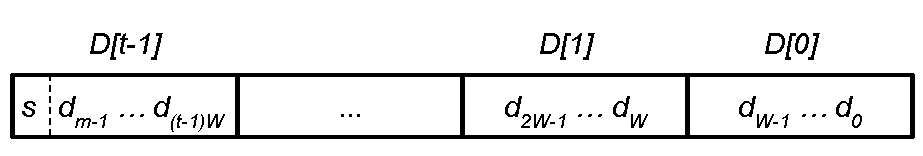
\includegraphics[width = .90\columnwidth]{figures/element-word.pdf}
\end{figure}

This operation has some important practical applications. Using a trinomial as irreducible polynomial is preferred when available because it maximizes the number of zero coefficients in the the irreducible polynomial, enabling numerous simplifications. And the reduction operation is an important step for multiplications and exponentiations, making speedups desirable.\\

This chapter requires more notations and assumptions to represent CPU algorithms and words. We assume that one word has $W$ bits, where $W$ is a multiple of $8$. The bits of a word $A$ are numbered from $0$ to $W-1$, with the rightmost bit corresponding to the $x^0$ coefficient (LSB) of $A$ designated as bit $0$. The following standard notation is used to denote operations on words $A$ and $B$:\\

\begin{description}
\item[$A \BitXOR B$] bitwise exclusive or.
\item[$A \BitOr B$]  bitwise or. 
\item[$A \BitAnd B$]      bitwise $AND$.
\item[$A \ShiftLeft n$]      left shift of $A$ by $n$ positions, ($n<W$), with the bits from 0 to $n-1$ set to $0$. 
\item[$A\ShiftRight n$]     righ shift of $A$ by $n$ positions, ($n<W$), with bits from $W-n$ to $W-1$ set to $0$. 
\end{description}

And the following variable naming:

\begin{description}
\item[$a, b, c, d$]  Polynomials in $\F_2[x]$, not necessarily an element of the field $\F_{2^m}$ (they may be an intermediate result before the final reduction).
\item[$A, B, C, D$]  Vector of bits corresponding to the polynomials $a, b, c, d$.
\end{description}

In Section~\ref{operating-on-words} we give more details on the general differences of bit and word algorithms for this application. Section~\ref{delay-independence} shows an example of such difference. Section~\ref{bit-grouping} details the different cases of bit-grouping and how they lie across word boundaries. Section~\ref{helper-functions} contains helper functions that can be used to easily convert a bit-oriented algorithm to a word-oriented one.

\section{Operating on words}\label{operating-on-words}

Manipulation of individual bits is not efficient in most CPU architectures. In general, it is preferred to operate on words, with a size specific to the microprocessor architecture, such as $32$- or $64$-bit words. However, the reduction algorithms are strongly bit oriented, since the coefficients are not naturally grouped in words. The codification of these algorithms to word oriented programming languages usually adds some complexity in terms of bitwise shifts and masks, and doesn't enjoy the parallelism inherent in XOR circuits. Specific techniques that help us in this coding have been proposed in the literature\cite{Hilewitz2008}.  \\

In this scenario it's often desirable to have "interoperability", choosing a field size and a irreducible polynomial that leads to efficient operations in both hardware and software implementations. A straightforward approach to this problem is to develop a hardware implementation first, XOR'ing individual bits, and convert the algorithm to words. This can be thought of as parallelizing the operations, with SHIFTs and AND/OR masks for alignment. This is the approach used in this work. \\

The difficulty of the conversion process greatly varies depending on the access pattern of the algorithm and alignment of words. If all coefficients inside a range are XOR'ed once in a linear fashion, the XOR distance a multiple of the word size, and the start and end range lie in word boundaries, the converted algorithm gains a full speedup of up to \texttt{WORD\_SIZE} times {[}$C_{word} = \ceil*{\frac{C_{bit}}{W}}${]}. \\

The word-oriented algorithm can be helped by choosing specific field sizes and irreducible polynomials that introduce operations aligning at word boundaries, to avoid these bitwise shifts and masks, or that map well to architecture-specific operations. In our algorithms we try to make use of alignment opportunities when they appear, but do not depend on them or any specific architecture. \\

\section{Delay independence}\label{delay-independence}

Performing binary polynomial reduction in a CPU has a few differences from implementing a hardware circuit. For example, circuits often avoid irreducible polynomials with the second largest exponent $a > \ceil{m/2}$. As seen before with pentanomials, this characteristic leads to higher delays in most circuit-based reduction algorithms. This is caused by the inter-dependency of the calculations, limiting the natural parallelism of circuits and thus increases the total delay. \\

This property does not affect software implementations. To illustrate this, we take two algorithms that perform modular reduction for the NIST irreducible trinomials $x^{233} + x^{74} + 1$ and $x^{409} + x^{87} + 1$~\cite[p. 55]{hankerson2006guide}. Then we manually adapt each of these algorithms to perform a reduction modulo its reciprocal, $x^m + x^{a-m} + 1$. Notice the only change required is in the indexing and bitwise shifts. The total number of operations remains the same. Algorithms meant for circuit implementations, on the other hand, would have different delay characteristics on each version. \\ % Muito pouco. Expandir. Mostrar diferenças linha-a-linha.

% Explicar melhor os algoritmos.

% Exemplos de execução (olhar no livro do hankerson)

% Tabela comparando custo para deixar explícito que o custo é o mesmo.

\begin{algorithm}
\begin{algorithmic}[1]
  \REQUIRE $C[2m-2,0]$
  \ENSURE $C[m-1,0]$
  \FOR{$i \gets 15$ \textbf{downto} $8$}
    \STATE $T \gets C[i]$
    \STATE $C[i-8] \gets C[i-8] \oplus T << 23$
    \STATE $C[i-7] \gets C[i-7] \oplus T >> 9$
    \STATE $C[i-5] \gets C[i-5] \oplus T << 1$
    \STATE $C[i-4] \gets C[i-4] \oplus T >> 31$
  \ENDFOR
  \STATE $T \gets C[7] >> 9$
  \STATE $C[0] \gets C[0] \oplus T$
  \STATE $C[2] \gets C[2] \oplus T << 10$
  \STATE $C[3] \gets C[3] \oplus T >> 22$
  \STATE $C[7] \gets C[7] \& \texttt{0x1FF}$
  \RETURN $C$
  \caption{Hankerson's algorithm for reduction modulus $x^{233} + x^{74} + 1$, a standardized NIST polynomial.}
  \label{alg:233_74_nist}
\end{algorithmic}
\end{algorithm}

 \begin{algorithm}
 \begin{algorithmic}[1]
  \REQUIRE $C[2m-2,0]$
  \ENSURE $C[m-1,0]$
  \FOR{$i \gets 14$ \textbf{downto} $8$}
    \STATE $T \gets C[i]$
    \STATE $C[i-8] \gets C[i-8] \oplus T << 23$
    \STATE $C[i-7] \gets C[i-7] \oplus T >> 9$
    \STATE $C[i-3] \gets C[i-3] \oplus T << 22$
    \STATE $C[i-2] \gets C[i-2] \oplus T >> 10$
  \ENDFOR
  \STATE $T \gets C[7] >> 9$
  \STATE $C[0] \gets C[0] \oplus T$
  \STATE $C[2] \gets C[2] \oplus T << 31$
  \STATE $C[3] \gets C[3] \oplus T >> 1$
  \STATE $C[7] \gets C[7] \& \texttt{0x1FF}$
  \RETURN $C$
  \caption{Algorithm for reduction modulus $x^{233} + x^{159} + 1$, $(233, 74)$'s recriprocal.}
  \label{alg:233_159}
\end{algorithmic}
\end{algorithm}

\begin{algorithm}
\begin{algorithmic}[1]
  \REQUIRE $C[2m-2,0]$
  \ENSURE $C[m-1,0]$
  \FOR{$i \gets 25$ \textbf{downto} $13$}
    \STATE $T \gets C[i]$
    \STATE $C[i-13] \gets C[i-13] \oplus T << 7$
    \STATE $C[i-12] \gets C[i-12] \oplus T >> 25$
    \STATE $C[i-11] \gets C[i-11] \oplus T << 30$
    \STATE $C[i-10] \gets C[i-10] \oplus T >> 2$
  \ENDFOR
  \STATE $T \gets C[12] >> 25$
  \STATE $C[0] \gets C[0] \oplus T$
  \STATE $C[2] \gets C[2] \oplus T << 23$
  \STATE $C[12] \gets C[12] \& \texttt{0x1FFFFFF}$
  \RETURN $C$
  \caption{Hankerson's algorithm for reduction modulus $x^{409} + x^{87} + 1$, a standardized NIST polynomial.}
  \label{alg:409_87_nist}
\end{algorithmic}
\end{algorithm}


\begin{algorithm}
\begin{algorithmic}[1]
  \REQUIRE $C[2m-2,0]$
  \ENSURE $C[m-1,0]$
  \FOR{$i \gets 25$ \textbf{downto} $13$}
    \STATE $T \gets C[i]$
    \STATE $C[i-13] \gets C[i-13] \oplus T << 7$
    \STATE $C[i-12] \gets C[i-12] \oplus T >> 25$
    \STATE $C[i-3] \gets C[i-3] \oplus T << 9$
    \STATE $C[i-2] \gets C[i-2] \oplus T >> 23$
  \ENDFOR
  \STATE $T \gets C[12] >> 25$
  \STATE $C[0] \gets C[0] \oplus T$
  \STATE $C[10] \gets C[10] \oplus T << 2$
  \STATE $C[12] \gets C[12] \& \texttt{0x1FFFFFF}$
  \RETURN $C$
  \caption{Algorithm for reduction modulus $x^{409} + x^{322} + 1$, $(409, 87)$'s reciprocal.}
  \label{alg:409_322}
\end{algorithmic}
\end{algorithm}

\section{Bit grouping}\label{bit-grouping}

Figure~\ref{fig:elemento:field} shows the representation of a element $d \in \ftwom$ as an array $D$ of $t$ words of $W$ bits, where $t = \left \lceil \frac{m}{W} \right \rceil$. The $s = tW-m$ highest order bits of $D[t-1]$ are not unused.
\begin{figure}[htb]
  \centering
  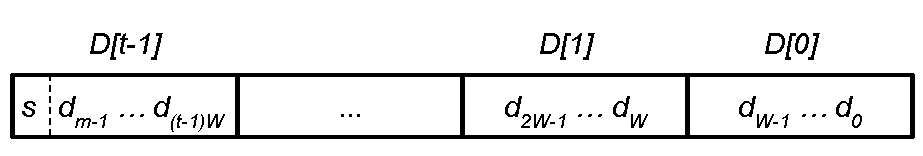
\includegraphics[width = .55\columnwidth]{figures/element-word.pdf}
\caption{Representation of $d \in \ftwom$ as an array $D$ of $W$ bit words. The $s = tW-m$ highest order bits of $D[t-1]$ are not unused.}
\label{fig:elemento:field}
\end{figure}
\\

For the case where $(m-1) \mod{W} > \frac{W}{2}$, the Figure~\ref{fig:elemento:field:mult} shows the representation of an element $d = ab$, $a,b \in \ftwom$ as an array $D$ of $W$-bit words. The $s = 2(tW-m)+1$ highest order bits of $D[2t-1]$ are not unused.

\begin{figure}
  \centering
  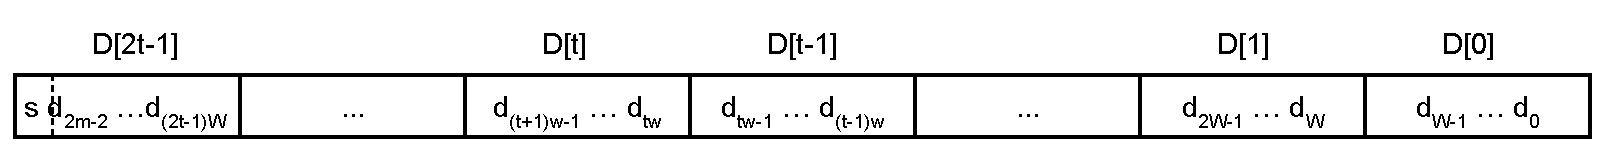
\includegraphics[width = .9\columnwidth]{figures/two-word-element-1.pdf}
\caption{Representation of $d = ab$, $a,b \in \ftwom$ as an array $D$ of $W$-bit words. The $s = 2(tW-m)+1$ highest order bits of $D[2t-1]$ are not unused.}
\label{fig:elemento:field:mult}
\end{figure}


When $(m-1) \mod{W} \leq \frac{W}{2}$, $D[2t-1]$ is not needed.  Figure~\ref{fig:elemento:field:mult2} shows the representation of a element $d = ab$, $a,b \in \ftwom$ as an array $D$ of $W$-bit words. The $s = 2(tW-m)+1$ highest order bits of $D[2t-2]$ and $D[2t-1]$ are not unused.
\begin{figure}
  \centering
  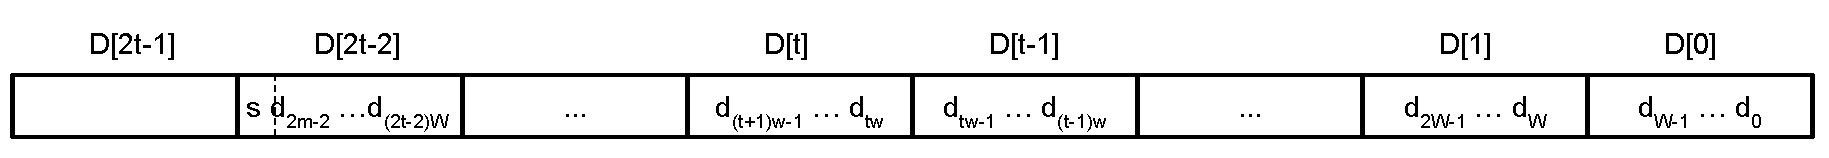
\includegraphics[width = \columnwidth]{figures/two-word-element-2.pdf}
\caption{Representation of $d = ab$, $a,b \in \ftwom$ as an array $D$ of $W$-bit words. The $s = 2(tW-m)+1$ highest order bits of $D[2t-2]$ and $D[2t-1]$ are not unused.}
\label{fig:elemento:field:mult2}
\end{figure}

In these cases a whole word is wasted, but length calculations become simpler: to get the length (in words) of a product of two elements, just add their lengths (in words).


\section{Helper functions for conversion} \label{helper-functions}

The word-oriented versions of the algorithm can be created by noticing the bit access pattern. The XOR operation pattern can be thought of XORing two ranges.

Each of them perform a XOR operation between all bits in a certain range and counterparts a fixed distance away. This access pattern allows word-level parallelism. There are four issues that need to be paid attention to:

\textbf{Misaligned start:}
The loop starts at $2m -2$, which may not align with the word length ($W \nmid 2m-2$). To avoid overwriting the upper bits of this incomplete word we must clear them from the \texttt{src} word.

\textbf{Misaligned ends:}
The fix is identical to the misaligned start, where we clear the extra bits from the incoming word.

\textbf{Misaligned source:}
The source/incoming word may not be aligned to word boundaries either. In this case we need to pull bits from the next word too, shifting both of them for correct placement. Unfortunately this issue affects the start and ends word too, further complicating their treatment.

\textbf{Too small distances:}
Finally, if the distance between the XOR'ed words ($m-a$, $m$, respectively) is smaller than $W/2$, the same bit will be written and read in the same word-step. This is not possisble with a single operation, and requires handling each word in mulitple parts. This is suboptimal and should be avoided by better choices of $m$, $a$ and $W$.

Other bit-level operations are emulated with word masks and shifts.

To help transforming an algorithm in its word-parallel version we introduce the following helper functions. Notice the function calls can be inlined and all conditionals are open for static analysis (the final algorithm should contain no conditionals if optimized properly).

\begin{algorithm}
\begin{algorithmic}[1]
  \REQUIRE $dst$, $src$, $W$, $C[]$
  \STATE $mask \gets 1 << (src \mod W)$
  \STATE $C[dst / W] \gets C[dst / W] \oplus (C[src / W] \land mask) << (dst \mod W - src \mod W)$
  \caption{\texttt{XOR\_BIT}: Single bit XOR inside word}
\end{algorithmic}
\end{algorithm}

\begin{algorithm}
\begin{algorithmic}[1]
  \REQUIRE $dst$, $src$, $W$, $C[]$
  \STATE $left \gets C[src / W] >> (src \mod W)$
  \STATE $right \gets C[src / W + 1] << (W - src \mod W)$
  \STATE $C[dst / W] \gets C[dst / W] \oplus (left \lor right)$
  \caption{\texttt{XOR\_WORD}: Whole word XOR with possibly misaligned source}
\end{algorithmic}
\end{algorithm}

\begin{algorithm}
\begin{algorithmic}[1]
  \REQUIRE $dst$, $src$, $n\_bits$, $W$, $C[]$
  \STATE $shift \gets src \mod W$
  \STATE $left\_n\_bits \gets \min(n\_bits, W - shift)$
  \STATE $leftmask \gets ((1 << left\_n\_bits) - 1) << shift$
  \STATE $left \gets (C[src / W] \land leftmask) >> shift$
  \STATE $right\_n\_bits \gets n\_bits - left\_n\_bits$
  \IF{$right\_n\_bits > 0$}
    \STATE $rightmask \gets (1 << right\_n\_bits) - 1$
    \STATE $right \gets (C[src/W+1] \land rightmask) << left\_n\_bits$
  \ELSE
    \STATE $right \gets 0$
  \ENDIF
  \STATE $C[dst/W] = C[dst/W] \oplus ((left | right) << (dst \ W))$
  \caption{\texttt{XOR\_PARTIAL\_WORD}: XOR a range of bits inside a word, with possibly misaligned source}
\end{algorithmic}
\end{algorithm}

\begin{algorithm}
\begin{algorithmic}[1]
  \REQUIRE $start\_dst$, $end\_dst$, $distance$, $W$, $C[]$
  \IF{$end\_dst/W = start\_dst/W$}
    \STATE \texttt{XOR\_PARTIAL\_WORD}($start\_dst$, $start\_dst + distance$, $end\_dst - start\_dst$, $W$, $C$)
  \ELSE
    \IF{$start\_dst \ W \neq 0$}
      \STATE $remaining = W - (start\_dst \ W)$
      \STATE \texttt{XOR\_PARTIAL\_WORD}($start\_dst$, $start\_dst + distance$, $remaining$, $W$, $C$)
      \STATE $start\_dst \gets start\_dst + remaining$
    \ENDIF
    
    \STATE $rounded\_end \gets (end\_dst / W) * W$
    \STATE $dst \gets start\_dst$
    \WHILE{$dst < rounded\_end$}
      \STATE \texttt{XOR\_WORD}($dst$, $dst + distance$, $W$, $C$)
      \STATE $dst \gets dst + W$
    \ENDWHILE
    
    \IF{$end\_dst \ W \neq 0$}
      \STATE \texttt{XOR\_PARTIAL\_WORD}($rounded\_end$, $rounded\_end + distance$, $end\_dst \ W$, $W$, $C$)
    \ENDIF
  \ENDIF
  \caption{\texttt{XOR\_RANGE}: XOR a range of bits (across many words) with an equivalent range a certain distance away}
\end{algorithmic}
\end{algorithm}


And the word-transformed algorithms are:

\begin{algorithm}
\begin{algorithmic}[1]
  \REQUIRE $m$, $a$, $W$, $C\left[0,\ceil*{\frac{2m-2}{W}}\right]$
  \ENSURE $C[0,m-1]$
  \STATE \texttt{XOR\_RANGE}($a$, $a+m$, $m$, $W$, $C$)
  \STATE \texttt{XOR\_RANGE}($0$, $a-1$, $m$, $W$, $C$)
  \RETURN $C$
  \caption{Simple word-parallel reduction algorithm for $x^m + x^a +1$, $a = \frac{m}{2}$}
  \label{alg:equallyspaced:word:operation}
\end{algorithmic}
\end{algorithm}

\begin{algorithm}
\begin{algorithmic}[1]
  \REQUIRE $m$, $a$, $W$, $C\left[0,\ceil*{\frac{2m-2}{W}}\right]$
  \ENSURE $C[0,m-1]$
  \STATE $start\_src \gets m$
  \STATE $step\_size \gets m - a$
  \WHILE{$start\_src \le 2m - 2$}
    \STATE \texttt{XOR\_RANGE}($a$, $a + 2m-2 - start\_src$, $start\_src - a$, $W$, $C$)
    \STATE $start\_src \gets start\_src + step\_size$
    \STATE $step\_size \gets 2 \times step\_size$
  \ENDWHILE
  \STATE \texttt{XOR\_RANGE}($0$, $m$, $m$, $W$, $C$)
  \RETURN $C$
  \caption{Alternative reduction algorithm, uses more XORs but less calls to \texttt{XOR\_RANGE}, may be useful for certain architectures.}
  \label{alg:new:word:operation}
\end{algorithmic}
\end{algorithm}


The algorithm \ref{alg:new:word:operation} proposed can be applied to specific trinomials with fixed parameters. For example, for the commonly used field $x^{233} + x^{74} + 1$, with 32-bit words, this results in algorithm \ref{alg:233-32:word:operation}. The total number of operations of this algorithm is 19 XORs, 16 ORs, 5 ANDs and 35 shifts, for a total of 75 word operations.

\begin{algorithm}
\begin{algorithmic}[1]
  \REQUIRE $C\left[0,\ceil*{\frac{2m-2}{W}}\right]$
  \ENSURE $C[0,m-1]$
  \STATE $C[2] \gets C[2] \oplus ((C[7] \land \texttt{0x7ffffe00}) << 1)$
  \STATE $C[3] \gets C[3] \oplus ((C[7] >> 31) \lor (C[8] << 1))$
  \STATE $C[4] \gets C[4] \oplus ((C[8] >> 31) \lor (C[9] << 1))$
  \STATE $C[5] \gets C[5] \oplus ((C[9] >> 31) \lor (C[10] << 1))$
  \STATE $C[6] \gets C[6] \oplus ((C[10] >> 31) \lor (C[11] << 1))$
  \STATE $C[7] \gets C[7] \oplus ((C[11] >> 31) \lor (C[12] << 1))$
  \STATE $C[8] \gets C[8] \oplus ((C[12] >> 31) \lor (C[13] << 1))$
  \STATE $C[9] \gets C[9] \oplus ((C[13] >> 31) \lor ((C[14] \land \texttt{0x1ffff}) >> 1))$
  \STATE $C[2] \gets C[2] \oplus ((C[12] \land \texttt{0x3fffff00}) << 2)$
  \STATE $C[3] \gets C[3] \oplus ((C[12] >> 30) \lor (C[13] << 2))$
  \STATE $C[4] \gets C[4] \oplus ((C[13] >> 30) \lor ((C[14] \land \texttt{0x1ffff}) >> 2))$
  \STATE $C[0] \gets C[0] \oplus ((C[7] >> 9) \lor (C[8] << 23))$
  \STATE $C[1] \gets C[1] \oplus ((C[8] >> 9) \lor (C[9] << 23))$
  \STATE $C[2] \gets C[2] \oplus ((C[9] >> 9) \lor (C[10] << 23))$
  \STATE $C[3] \gets C[3] \oplus ((C[10] >> 9) \lor (C[11] << 23))$
  \STATE $C[4] \gets C[4] \oplus ((C[11] >> 9) \lor (C[12] << 23))$
  \STATE $C[5] \gets C[5] \oplus ((C[12] >> 9) \lor (C[13] << 23))$
  \STATE $C[6] \gets C[6] \oplus ((C[13] >> 9) \lor (C[14] << 23))$
  \STATE $C[7] \gets C[7] \oplus ((C[14] \land \texttt{0x3fe00}) >> 9)$
  \RETURN $C$
  \caption{Reduction algorithm for $x^{233} + x^{74} + 1$ with 32-bit words}
  \label{alg:233-32:word:operation}
\end{algorithmic}
\end{algorithm}

% "joguinho" boppreh.com
\chapter{Visual debugger}
%\section{Introduction}

While studying binary reduction algorithms, we tested some cases by hand. However, even small polynomials can require dozens of bit operations, so the number and size of our manual tests was severely limited, but still yielded interesting results. \\

In our tests we often spotted interesting behaviors. Some bits would cancel themselves in ways that suggested a pattern, or a change in one of the variables would lead to non-obvious changes in the number of operations. On one hand, we knew many of those behaviors were coincidences, so attempts at extracting mathematical proofs for each of them would lead to many dead ends and wasted time. On the other hand, patterns like these were the base of many optimizations. \\

Therefore we needed a way to quickly test different parameters, and have the results be visually intuitive, in order to discern behaviors that were more likely to be useful. This chapter explains the initial process and the final tool developed. In Section~\ref{section:visual:manual} we explain how the manual tests were organized. Section~\ref{section:visual:alt} we show how the manual tests were reworked to create more visually intuitive results. Finally, Section~\ref{section:visual:final} contains some of the optimizations made for faster feedback, along with a few of the patterns observed. Section~\ref{section:visual:conclusion} concludes with some remarks.

\section{Manual reduction algorithm} \label{section:visual:manual}

The reduction process for polynomials in $GF(2^m)$ depends on two values: the irreducible polynomial $f(x) = x^m + x^a + ... + 1$, and the value to be reduced, $C(x) = \sum_{i=0}^{d} c_i x^i$, $d \geq m$. Here we focus on the common case $d=2m-2$, where $C$ is the product of two polynomials of degree $m$, or the square of a single polynomial of this size. \\

For example, take the irreducible trinomial $f(x) = x^7 + x^3 + 1$, and $C(x) = x^{12} + x^{10} + x^9 + x^7 + x^6 + x^3 + x^2 + 1$. We can look at $f$ and $C$ as arrays of bits (see Figure~\ref{fig:visual:table_simplest}). \\

\begin{figure}
  \centering
\begin{TAB}(e){|c|c|c|c|c|c|c|c|c|c|c|c|c|}{|c|c|c|}
\emph{$x^{12}$} & \emph{$x^{11}$} & \emph{$x^{10}$} & \emph{$x^9$} & \emph{$x^8$} & \emph{$x^7$} & \emph{$x^6$} & \emph{$x^5$} & \emph{$x^4$} & \emph{$x^3$} & \emph{$x^2$} & \emph{$x^1$} & \emph{$x^0$} \\
  &   &   &   &   & 1 & 0 & 0 & 0 & 1 & 0 & 0 & 1 \\
1 & 0 & 1 & 1 & 0 & 1 & 1 & 0 & 0 & 1 & 1 & 0 & 1
\end{TAB}
\caption{The polynomials $x^7 + x^3 + 1$, and $x^{12} + x^{10} + x^9 + x^7 + x^6 + x^3 + x^2 + 1$ seen as arrays of bits.}
\label{fig:visual:table_simplest}
\end{figure}

At this point in the research, the algorithm we were using for polynomial reduction was slightly different from the one previously shown. First, notice that $0 \equiv f \mod f$, so we can add $f$ or any multiple to an expression. The reduction algorithm then consists of, for each term $c_i x^i,~i \geq deg(f)$, adding $c_{i} x^{i-m} f(x)$. By adding $c_i x^{i}$ we are canceling that term, and the other terms added have degree strictly smaller than the one canceled. \\

Notice, however, that while the other terms added have a smaller degree, they may still require further reduction. Therefore the algorithm is repeated until all remaining terms have degree smaller than the irreducible polynomial. \\

Let's apply this algorithm to our example, $C(x) = x^{12} + x^{10} + x^9 + x^7 + x^6 + x^3 + x^2 + 1$ and $f(x) = x^7 + x^3 + 1$. The first step is to take the terms of $C$ that have degree 7 or higher, and add three copies: $c_i x^i$ itself, $c_i x^{i-7+3}$ and $c_i x^{i-7}$. Figure~\ref{fig:visual:old_first} shows this first step. The first six elements have degree greater than or equal to 7 ,and required reduction, so three copies were created, multiplied by different amounts. The result of this first step is the column-wise XOR, shown after the dashed line.\\

\begin{figure}
  \centering
\begin{TAB}(e){|c|c|c|c|c|c|c|c|c|c|c|c|c|}{|c|c|c|c|c:c|}
\emph{$x^{12}$} & \emph{$x^{11}$} & \emph{$x^{10}$} & \emph{$x^9$} & \emph{$x^8$} & \emph{$x^7$} & \emph{$x^6$} & \emph{$x^5$} & \emph{$x^4$} & \emph{$x^3$} & \emph{$x^2$} & \emph{$x^1$} & \emph{$x^0$} \\
\textbf{1} & \textbf{0} & \textbf{1} & \textbf{1} & \textbf{0} & \textbf{1} & 1 & 0 & 0 & 1 & 1 & 0 & 1 \\
  1 & 0 & 1 & 1 & 0 & 1 &   &   & &   &   &   &  \\
  &   &   &   & 1 & 0 & 1 & 1 & 0 & 1 &   &   &   \\
  &   &   &   &   &   &   & 1 & 0 & 1 & 1 & 0 & 1 \\
0 & 0 & 0 & 0 & 1 & 0 & 0 & 0 & 0 & 1 & 0 & 0 & 0
\end{TAB}
\caption{First step of the old, manual reduction algorithm, for the polynomial $x^{12} + x^{10} + x^9 + x^7 + x^6 + x^3 + x^2 + 1$ and irreducible polynomial $x^7 + x^3 + 1$.}
\label{fig:visual:old_first}
\end{figure}

Note the term $x^8$ is present, so further reduction is necessary. The algorithm is repeated, and the full process is visible in Figure~\ref{fig:visual:old_all}. Three new copies are created, but this time only for the terms $x^8$ and $x^7$, since all others must have been eliminated. The column-wise XOR shows the final result: $C(x) \equiv x^4 + x^3 + x \mod f(x)$. \\

\begin{figure}
  \centering
\begin{TAB}(e){|c|c|c|c|c|c|c|c|c|c|c|c|c|}{|c|c|c|c|c|c|c|c:c|}
\emph{$x^{12}$} & \emph{$x^{11}$} & \emph{$x^{10}$} & \emph{$x^9$} & \emph{$x^8$} & \emph{$x^7$} & \emph{$x^6$} & \emph{$x^5$} & \emph{$x^4$} & \emph{$x^3$} & \emph{$x^2$} & \emph{$x^1$} & \emph{$x^0$} \\
\textbf{1} & \textbf{0} & \textbf{1} & \textbf{1} & \textbf{0} & \textbf{1} & 1 & 0 & 0 & 1 & 1 & 0 & 1 \\
1 & 0 & 1 & 1 & 0 & 1 &   &   & &   &   &   &  \\
  &   &   &   & \textbf{1} & \textbf{0} & 1 & 1 & 0 & 1 &   &   &   \\
  &   &   &   &   &   &   & 1 & 0 & 1 & 1 & 0 & 1 \\
  &   &   &   & 1 & 0 &   &   &   &   &   &   &   \\
  &   &   &   &   &   &   &   & 1 & 0 &   &   &   \\
  &   &   &   &   &   &   &   &   &   &   & 1 & 0 \\
0 & 0 & 0 & 0 & 0 & 0 & 0 & 0 & 1 & 1 & 0 & 1 & 0
\end{TAB}
\caption{All two steps of the old, manual reduction algorithm, for the polynomial $x^{12} + x^{10} + x^9 + x^7 + x^6 + x^3 + x^2 + 1$ and irreducible polynomial $x^7 + x^3 + 1$.}
\label{fig:visual:old_all}
\end{figure}

The resulting visualization gives some insight into the algorithm, but is obscured by specific values used in this example. A more general visualization is possible, where the coefficients are simply numbered. Figure~\ref{fig:visual:old_all_generic} shows the case for a generic reduction modulo $x^7 + x^3 + 1$. For example, the term $x^2$ of the output is the XOR of the terms $x^2$ and $x^9$ of the input. \\

\begin{figure}
  \centering
\begin{TAB}(e){|c|c|c|c|c|c|c|c|c|c|c|c|c|}{|c|c|c|c|c|c|c|c|}
\emph{$x^{12}$} & \emph{$x^{11}$} & \emph{$x^{10}$} & \emph{$x^9$} & \emph{$x^8$} & \emph{$x^7$} & \emph{$x^6$} & \emph{$x^5$} & \emph{$x^4$} & \emph{$x^3$} & \emph{$x^2$} & \emph{$x^1$} & \emph{$x^0$} \\
\textbf{12} & \textbf{11} & \textbf{10} & \textbf{9} & \textbf{8} & \textbf{7} & 6 & 5 & 4 & 3 & 2 & 1 & 0 \\
12& 11& 10& 9 & 8 & 7 &   &   & &   &   &   &  \\
  &   &   &   & \textbf{12} & \textbf{11} & 10& 9 & 8 & 7 &   &   &   \\
  &   &   &   &   &   &   & 12& 11& 10& 9 & 8 & 7 \\
  &   &   &   & 12& 11&   &   &   &   &   &   &   \\
  &   &   &   &   &   &   &   & 12& 11&   &   &   \\
  &   &   &   &   &   &   &   &   &   &   & 12& 11\\
\end{TAB}
\caption{All two steps of the old, manual reduction algorithm, for a generic polynomial and irreducible polynomial $x^7 + x^3 + 1$.}
\label{fig:visual:old_all_generic}
\end{figure}

This visual representation was our main exploration tool during the beginning of the research. Unfortunately it quickly gets unwieldy. The number of columns is $2m-2$, so visualizing large irreducible polynomials creates numerous small cells with unreadable contents. Furthermore, tables like these take some time to build by hand, and it's hard to spot patterns in the cell numbers. \\


\section{Alternative visualization tool} \label{section:visual:alt}

Tables like Figure~\ref{fig:visual:old_all_generic} some time to build by hand, but the process is easy to automate. A Javascript prototype was created, where HTML tables were built automatically for a given irreducible polynomial. This saved time, but did not make the result more readable. Large stables still had had the problem of small cells being unreadable, and spotting numeric patterns continued to be challenging. \\

The next step was to notice that the order of the steps does not matter, and neither does the grouping of operations in rows. For example, for the column $x^2$, as long as the inputs for $c_2$ and $c_9$ were XOR-ed together, the result would be correct. That is to say, the table visualization is stateless. \\

Based on this property, an alternative visualization was quickly discovered: making the table square, and numbering the rows instead of numbering the cells. By the old method, placing the numbers $2$ and $9$ anywhere in the column $x^2$, indicates that the $c_2$ coefficient should be XOR-ed with $c_9$ to produce the output corresponding to the term $x^2$. In the new visualization, instead of writing the numbers $2$ and $9$, the rows indicated by $c_2$ and $c_9$ are filled with some binary mark. \\

Figure~\ref{fig:visual:new} shows an example of this visualization, using $\oplus$ to mark the cells that should be XOR-ed (column-wise) to create the output. First, note that the columns $x^7 \ldots x^{12}$ are empty, as expected for a reduction algorithm. In the old visualization, the column $x^7$, for example, contained the number $7$ twice and the number $11$ twice. The result of these XOR operations is zero, but to arrive at this conclusion one has to go through the values and match the pairs. In the new visualization, cancellations like this are readily apparent because the cells are empty. \\

Furthermore, the two steps of the algorithm are still visible as two pairs of diagonal lines. The first step is a pair of diagonal lines going from $(c_7,~x^0)$ to $(c_{12}~,x^5)$ (from the constant term of the irreducible polynomial), and from $(c_7~,x^3)$ until being cut-off at $(c_{10},~x^6)$ (from the $x^3$ term of the irreducible polynomial). The second step is represented by the pair of diagonal lines from $(c_{11},~x^0)$ to $(c_{12},~x^1)$, and from $(c_{11},~x^3)$ to $(c_{12},~x^4)$. \\

\begin{figure}
  \centering
\begin{TAB}(e){|c|c|c|c|c|c|c|c|c|c|c|c|c|c|}{|c|c:c:c:c:c:c:c:c:c:c:c:c:c|}
& \emph{$x^{12}$} & \emph{$x^{11}$} & \emph{$x^{10}$} & \emph{$x^9$} & \emph{$x^8$} & \emph{$x^7$} & \emph{$x^6$} & \emph{$x^5$} & \emph{$x^4$} & \emph{$x^3$} & \emph{$x^2$} & \emph{$x^1$} & \emph{$x^0$} \\
$c_{12}$ &   &   &   &   &   &   &   & $\oplus$ & $\oplus$ &   &   & $\oplus$ & \\
$c_{11}$ &   &   &   &   &   &   &   &   & $\oplus$ & $\oplus$ &   &   & $\oplus$\\
$c_{10}$ &   &   &   &   &   &   & $\oplus$ &   &   & $\oplus$ &   &   & \\
$c_9$    &   &   &   &   &   &   &   & $\oplus$ &   &   & $\oplus$ &   & \\
$c_8$    &   &   &   &   &   &   &   &   & $\oplus$ &   &   & $\oplus$ & \\
$c_7$    &   &   &   &   &   &   &   &   &   & $\oplus$ &   &   & $\oplus$\\
$c_6$    &   &   &   &   &   &   & $\oplus$ &   &   &   &   &   & \\
$c_5$    &   &   &   &   &   &   &   & $\oplus$ &   &   &   &   & \\
$c_4$    &   &   &   &   &   &   &   &   & $\oplus$ &   &   &   & \\
$c_3$    &   &   &   &   &   &   &   &   &   & $\oplus$ &   &   & \\
$c_2$    &   &   &   &   &   &   &   &   &   &   & $\oplus$ &   & \\
$c_1$    &   &   &   &   &   &   &   &   &   &   &   & $\oplus$ & \\
$c_0$    &   &   &   &   &   &   &   &   &   &   &   &   & $\oplus$
\end{TAB}
\caption{Improved visualization of a polynomial reduction modulo $x^7 + x^3 + 1$. Output is decided by column-wise XOR of the values indicated by the rows.}
\label{fig:visual:new}
\end{figure}

\section{section:visual:final}

The cut-off seen at column $x^7$ in Figure~\ref{fig:visual:new} is technically correct, but truncates patterns that could be useful if seen in full. For example, it's not clear if the diagonal $(c_7~,x^3)$ to $(c_{10},~x^6)$ would really continue if "given the chance", or if it naturally stopped at the column $x^6$. To have a more intuitive understanding of these patterns, we decided to use the tool without any truncation. Mathematically, this means adapting the algorithm to add $c_{i} x^{i-m} f(x) + x^{i}$. An example of this non-truncated visualization is Figure~\ref{fig:visual:new_full}. There we find our answer for the previous conundrum: the diagonal that was truncated really was supposed to continue.

\begin{figure}
  \centering
\begin{TAB}(e){|c|c|c|c|c|c|c|c|c|c|c|c|c|c|}{|c|c:c:c:c:c:c:c:c:c:c:c:c:c|}
& \emph{$x^{12}$} & \emph{$x^{11}$} & \emph{$x^{10}$} & \emph{$x^9$} & \emph{$x^8$} & \emph{$x^7$} & \emph{$x^6$} & \emph{$x^5$} & \emph{$x^4$} & \emph{$x^3$} & \emph{$x^2$} & \emph{$x^1$} & \emph{$x^0$} \\
$c_{12}$ & $\oplus$ &   &   &   & $\oplus$ &   &   & $\oplus$ & $\oplus$ &   &   & $\oplus$ & \\
$c_{11}$ &   & $\oplus$ &   &   &   & $\oplus$ &   &   & $\oplus$ & $\oplus$ &   &   & $\oplus$\\
$c_{10}$ &   &   & $\oplus$ &   &   &   & $\oplus$ &   &   & $\oplus$ &   &   & \\
$c_9$    &   &   &   & $\oplus$ &   &   &   & $\oplus$ &   &   & $\oplus$ &   & \\
$c_8$    &   &   &   &   & $\oplus$ &   &   &   & $\oplus$ &   &   & $\oplus$ & \\
$c_7$    &   &   &   &   &   & $\oplus$ &   &   &   & $\oplus$ &   &   & $\oplus$\\
$c_6$    &   &   &   &   &   &   & $\oplus$ &   &   &   &   &   & \\
$c_5$    &   &   &   &   &   &   &   & $\oplus$ &   &   &   &   & \\
$c_4$    &   &   &   &   &   &   &   &   & $\oplus$ &   &   &   & \\
$c_3$    &   &   &   &   &   &   &   &   &   & $\oplus$ &   &   & \\
$c_2$    &   &   &   &   &   &   &   &   &   &   & $\oplus$ &   & \\
$c_1$    &   &   &   &   &   &   &   &   &   &   &   & $\oplus$ & \\
$c_0$    &   &   &   &   &   &   &   &   &   &   &   &   & $\oplus$
\end{TAB}
\caption{Improved visualization of a polynomial reduction modulo $x^7 + x^3 + 1$, now without truncation.}
\label{fig:visual:new_full}
\end{figure}

Additionally, note that this visualization is not only a rearrangement of the cells from the old, manual visualization. We mentioned having to pair values to find cancellations, and this is clearly visible in cases other than the truncation. For example, take the irreducible trinomial $x^6+x^3+1$. Its reduction pattern, when visualized in the old manual way, results in Figure~\ref{fig:visual:old_spaced}. Meanwhile, the new, columns-and-rows visualization, results in Figure~\ref{fig:visual:new_spaced}. \\

In Figure~\ref{fig:visual:old_spaced} notice how columns $x^3$ and $x^4$ had the coefficients from $c_{9}$ and $c_{10}$ added twice, resulting in two cancellations. These cancellations can be inferred in Figure~\ref{fig:visual:old_spaced}, but are glaringly obvious in Figure~\ref{fig:visual:new_spaced}. In fact, one can intuitive understand them by thinking of the two pairs diagonals, and realizing when one the smaller ones (from the second reduction step) "collided" with one of the larger ones (from the first reduction step). The result is that the cells $(c_9,~x^3)$ and $(c_10,~x^4)$ are empty because they were filled twice. \\

\begin{figure}
  \centering
\begin{TAB}(e){|c|c|c|c|c|c|c|c|c|c|c|}{|c|c|c|c|c|c|c|c|}
\emph{$x^{10}$} & \emph{$x^9$} & \emph{$x^8$} & \emph{$x^7$} & \emph{$x^6$} & \emph{$x^5$} & \emph{$x^4$} & \emph{$x^3$} & \emph{$x^2$} & \emph{$x^1$} & \emph{$x^0$} \\
\textbf{10} & \textbf{9} & \textbf{8} & \textbf{7} & \textbf{6} & 5 & 4 & 3 & 2 & 1 & 0 \\
10& 9 & 8 & 7 & 6 &   & &   &   &   &  \\
  &   &  & 10 & 9 & 8 & 7 & 6 & 5 &   &   \\
  &   &   &   &   &   & 10& 9 & 8 & 7 & 6 \\
  &   &   &10 & 9 &   &   &   &   &   &   \\
  &   &   &   &   &   & 10& 9 &   &   &   \\
  &   &   &   &   &   &   &   &   & 10& 9 \\
\end{TAB}
\caption{All two steps of the old, manual reduction algorithm, for a generic polynomial and irreducible polynomial $x^6 + x^3 + 1$.}
\label{fig:visual:old_spaced}
\end{figure}

\begin{figure}
  \centering
\begin{TAB}(e){|c|c|c|c|c|c|c|c|c|c|c|c|}{|c|c:c:c:c:c:c:c:c:c:c:c|}
& \emph{$x^{10}$} & \emph{$x^9$} & \emph{$x^8$} & \emph{$x^7$} & \emph{$x^6$} & \emph{$x^5$} & \emph{$x^4$} & \emph{$x^3$} & \emph{$x^2$} & \emph{$x^1$} & \emph{$x^0$} \\
$c_{10}$ & $\oplus$ &          &          & $\oplus$ &          &          &          &          &          & $\oplus$ & \\
$c_9$    &          & $\oplus$ &          &          & $\oplus$ &          &          &          &          &          & $\oplus$ \\
$c_8$    &          &          & $\oplus$ &          &          & $\oplus$ &          &          & $\oplus$ &          & \\
$c_7$    &          &          &          & $\oplus$ &          &          & $\oplus$ &          &          & $\oplus$ & \\
$c_6$    &          &          &          &          & $\oplus$ &          &          & $\oplus$ &          &          & $\oplus$ \\
$c_5$    &          &          &          &          &          & $\oplus$ &          &          &          &          & \\
$c_4$    &          &          &          &          &          &          & $\oplus$ &          &          &          & \\
$c_3$    &          &          &          &          &          &          &          & $\oplus$ &          &          & \\
$c_2$    &          &          &          &          &          &          &          &          & $\oplus$ &          & \\
$c_1$    &          &          &          &          &          &          &          &          &          & $\oplus$ & \\
$c_0$    &          &          &          &          &          &          &          &          &          &          & $\oplus$
\end{TAB}
\caption{Improved visualization of a polynomial reduction modulo $x^7 + x^3 + 1$, now without truncation.}
\label{fig:visual:new_spaced}
\end{figure}

As to why the diagonals moved in a way that resulted in cancellations, we need a way to animate these tables. In the tool this is performed by the mouse scroll-wheel. Scrolling up increments the term $x^a$ in the irreducible polynomial, while scrolling down decrements it. Holding the shift key changes the $x^m$ term instead, the degree of the irreducible polynomial. With this instantaneous feedback one can quickly acquire intuitions on these patterns. For example, incrementing $a$ moves all but the first diagonal (at column $x^0$) one cell to the left. Decrementing $m$ has the same result. This is why the cancellation happened in the $x^6+x^3+1$ case: the diagonals from $x^7+x^3+1$ moved one cell to the left, and one small diagonals "collided" with the first (static) diagonal. \\

All this intuition is naturally very informal. Its main uses is as an exploration tool and as a counter proof searcher. The use as exploratory tool is very clear: just by scrolling the scroll wheel one patterns where diagonals cancel each out perfectly, or where an unexpectedly high number of diagonals appear. Both of these can then be proved by more standard mathematical tools. Meanwhile, it's use as counter proof searcher helped save time in trying to prove false properties. It's easy to search hundreds of polynomials, in a very short space of time, looking for a case where the hypothesis under study is false. \\

Finally, this visualization tool was made to include testing of algorithms. At first this was done by allowing the user to click on columns to XOR them, with the goal of taking the identity matrix and transforming into the matrices seen above. This resulted in a surprisingly fun game (see Figure~\ref{fig:game}), but was only feasible for small irreducible polynomials. The second feature added was a text box where the user could input a Javascript algorithm, then display the algorithm execution step by step (Figure~\ref{fig:source}). This feature was later expanded to include word-processing algorithms, non-square tables (for larger reductions), and reduction of squared polynomials. \\

\begin{figure}
  \caption{Game based on reduction algorithms for binary finite fields modulo an irreducible trinomial.}
  \label{fig:game}
  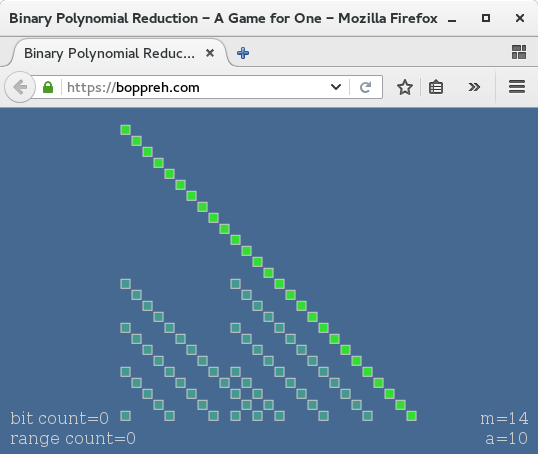
\includegraphics[width = .55\columnwidth]{figures/boppreh.png}
\end{figure}

\begin{figure}
  \caption{Visualization tool with input box for user algorithms.}
  \label{fig:source}
  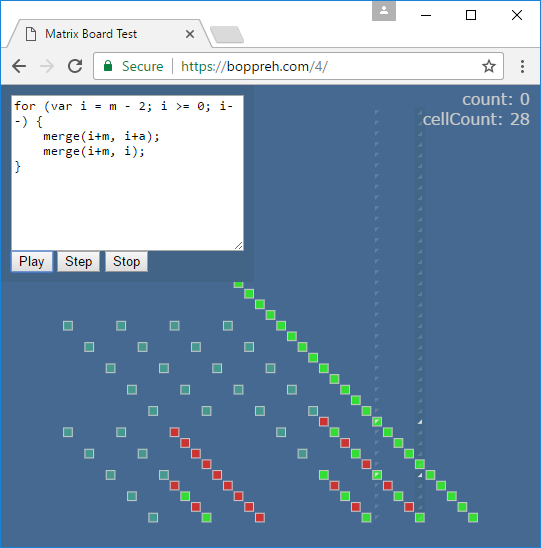
\includegraphics[width = .55\columnwidth]{figures/source.png}
\end{figure}


\section{Conclusion} \label{section:visual:conclusion}

In this chapter we presented the visualization tools used during our research. This tool was invaluable in efficiently exploring and testing new ideas related to reduction of binary polynomials. The intuitive visuals and quick feedback allowed even people unfamiliar with the subjects to help find interesting properties.

The development itself of the tool also acted to clarify concepts. For example the fact that each irreducible polynomial has a mathematical "pattern" associated, corresponding to the XORs required for reduction, and that these operations are independent of the algorithm used. The word processing and squaring versions saw less use, but creating them helped guide some of the research.

Interestingly, some time after having developed the tool, we found another researching using the same visualization of patterns, for the same problem.\cite{paper_com_imagens_dos_padroes}

% Discutir as contribuições. O que foi trazido de melhorias? Avaliação do trabalho. Contextualizar a contribuição, com análise crítical.
\chapter{Evalution?}
%\input{chapters/evaluation}

% Objetivos atingidos: específicos e gerais.
% Propostas futuras.
\chapter{Final considerations}
%% Relacionar os objetivos específicos ( cada um deles ) com o que foi feito e onde está isso no trabalho, de forma critica
% Trabalhos futuros: pelos menos apresentar 5 trabalhos futuros

\section{Conclusion} \label{conclusion}

In this work we present a low-complexity bit-parallel squarer algorithm. It is able to match the state of the art~\cite{wu2002bit} in XOR gate count when $GF(2^m)$ is defined using trinomials. Xiong~\cite{xiong2014gf} achieves lower XOR gate complexity when pentanomials are used; however it uses a special polynomial basis and is suitable to only a small fraction of all irreducible pentanomials, while ours is general for any low-weight polynomial.\\

Park~\cite{park2012explicit} also proposes a general squaring algorithm focusing on pentanomials with $a \leq \ceil{m/2}$. Her squarer is the best available in the literature considering both the number of XOR operations and the delay. However, our algorithm is able to match the circuit delay on some polynomials and has a strictly smaller number of XORs than the upper bound provided, while being suitable not only for pentanomials. 
We remark that our squarer works for any general low-weight $k$-nomial. As mentioned in Section~\ref{squaring} there is not much work in the literature for this type of $k$-nomial squarer, $k>5$, but our algorithm can still be efficiently used in these cases.\\

One disadvantage of our proposed squarer is that it may produce higher delays, up to $6 T_X$ for pentanomials. This can be mitigated in two ways. First, by narrowing the selection of irreducible pentanomial. Indeed,  pentanomials that result in a delay of $3 T_X$ are abundant. Second, the resulting circuit can be modified to reduce the delay in exchange for some extra XORs. An automated way to perform this tweak is still an open problem, as is the exact formula for circuit delays.\\

In conclusion, our algorithms give more freedom to select irreducible polynomials while maintaining competitive efficiency.





\section{References}

\bibliographystyle{ufsc-alf}
\bibliography{aaabibliografia}

\begin{appendices}

\section{Example of resulting algorithm}
\label{appendix:example}

\begin{algorithm}
\caption{Squaring for $\F_{2^{19}} \cong \F_2[x]/(x^{19} + x^5 + x^2 + x + 1)$}
\label{alg:square:example}
\begin{multicols}{2}
\begin{algorithmic}[1]
\REQUIRE $A = [a_0, a_1, a_2, ..., a_{18}]$, \\$f(x)~=~x^{19}~+~x^5~+~x^2~+~x~+~1$
\ENSURE $A^2 \mod f$
\STATE $C = [a_0, 0, a_1, 0, a_2, 0, \ldots, 0, a_{18}]$
\STATE $\mathbox{C[22]}{C[22]} \leftarrow C[22]  \oplus  C[36]$
\STATE $\mathbox{C[22]}{C[19]} \leftarrow C[36]$
\STATE $\mathbox{C[22]}{C[18]} \leftarrow C[18]  \oplus  C[36]$
\STATE $\mathbox{C[22]}{C[17]} \leftarrow C[36]$
\STATE $\mathbox{C[22]}{C[20]} \leftarrow C[20]  \oplus  C[34]$
\STATE $\mathbox{C[22]}{C[17]} \leftarrow C[17]  \oplus  C[34]$
\STATE $\mathbox{C[22]}{C[16]} \leftarrow C[16]  \oplus  C[34]$
\STATE $\mathbox{C[22]}{C[15]} \leftarrow C[34]$
\STATE $\mathbox{C[22]}{C[18]} \leftarrow C[18]  \oplus  C[32]$
\STATE $\mathbox{C[22]}{C[15]} \leftarrow C[15]  \oplus  C[32]$
\STATE $\mathbox{C[22]}{C[14]} \leftarrow C[14]  \oplus  C[32]$
\STATE $\mathbox{C[22]}{C[13]} \leftarrow C[32]$
\STATE $\mathbox{C[22]}{C[16]} \leftarrow C[16]  \oplus  C[30]$
\STATE $\mathbox{C[22]}{C[13]} \leftarrow C[13]  \oplus  C[30]$
\STATE $\mathbox{C[22]}{C[12]} \leftarrow C[12]  \oplus  C[30]$
\STATE $\mathbox{C[22]}{C[11]} \leftarrow C[30]$
\STATE $\mathbox{C[22]}{C[14]} \leftarrow C[14]  \oplus  C[28]$
\STATE $\mathbox{C[22]}{C[11]} \leftarrow C[11]  \oplus  C[28]$
\STATE $\mathbox{C[22]}{C[10]} \leftarrow C[10]  \oplus  C[28]$
\STATE $\mathbox{C[22]}{C[9]} \leftarrow C[28]$
\STATE $\mathbox{C[22]}{C[12]} \leftarrow C[12]  \oplus  C[26]$
\STATE $\mathbox{C[22]}{C[9]} \leftarrow C[9]  \oplus  C[26]$
\STATE $\mathbox{C[22]}{C[8]} \leftarrow C[8]  \oplus  C[26]$
\STATE $\mathbox{C[22]}{C[7]} \leftarrow C[26]$
\STATE $\mathbox{C[22]}{C[10]} \leftarrow C[10]  \oplus  C[24]$
\STATE $\mathbox{C[22]}{C[7]} \leftarrow C[7]  \oplus  C[24]$
\STATE $\mathbox{C[22]}{C[6]} \leftarrow C[6]  \oplus  C[24]$
\STATE $\mathbox{C[22]}{C[5]} \leftarrow C[24]$
\STATE $\mathbox{C[22]}{C[8]} \leftarrow C[8]  \oplus  C[22]$
\STATE $\mathbox{C[22]}{C[5]} \leftarrow C[5]  \oplus  C[22]$
\STATE $\mathbox{C[22]}{C[4]} \leftarrow C[4]  \oplus  C[22]$
\STATE $\mathbox{C[22]}{C[3]} \leftarrow C[22]$
\STATE $\mathbox{C[22]}{C[6]} \leftarrow C[6]  \oplus  C[20]$
\STATE $\mathbox{C[22]}{C[3]} \leftarrow C[3]  \oplus  C[20]$
\STATE $\mathbox{C[22]}{C[2]} \leftarrow C[2]  \oplus  C[20]$
\STATE $\mathbox{C[22]}{C[1]} \leftarrow C[20]$
\STATE $\mathbox{C[22]}{C[5]} \leftarrow C[5]  \oplus  C[19]$
\STATE $\mathbox{C[22]}{C[2]} \leftarrow C[2]  \oplus  C[19]$
\STATE $\mathbox{C[22]}{C[1]} \leftarrow C[1]  \oplus  C[19]$
\STATE $\mathbox{C[22]}{C[0]} \leftarrow C[0]  \oplus  C[19]$
\RETURN $C[0],~C[1],~C[2],~\ldots,~C[18]$
\end{algorithmic}
\end{multicols}
\end{algorithm}

Algorithm~\ref{alg:square:example} is an instance of Algorithm~\ref{alg:square}, wherein the irreducible polynomial is defined as $x^{19}+x^5+x^2+x+1$ by simply fixing $f$. We note the circuit has a delay of $3T_X$, due to the critical paths of the circuit lines $C[5]$ and $C[2]$. However, this value can be reduced with manual tweaks. By eliminating Lines 29, 31 and 38, and inserting $C[5] \leftarrow C[22] \oplus C[24]$ and $C[5] \leftarrow C[5] \oplus C[19]$ at the beginning, the delay of $C[5]$ is reduced to $2 T_X$ (and one XOR is saved). By moving Line 39 to before Line 36 the critical path of $C[2]$ is also reduced to only $2 T_X$, which becomes the total delay of the full circuit.

\end{appendices}

\end{document}
